\documentclass[output=paper]{langscibook}
\ChapterDOI{10.5281/zenodo.15006623}
\author{Chingduang Yurayong\orcid{}\affiliation{University of Helsinki; Mahidol University} and Saknarin Pimvunkum\affiliation{Mahidol University} and Yuttaporn Naksuk\affiliation{Mahidol University}}
\title[Convergence and divergence of tone paradigms across Tai dialects]
      {Convergence and divergence of tone paradigms across Tai dialects in the 21st century}
\abstract{The present study examines tone paradigms of Tai dialects spoken in Laos, Malaysia, Myanmar, Thailand, and Vietnam. The focus is on the homophones between the paradigmatic tone D in checked syllables and tones A, B, and C in smooth syllables. The method comprises a conventional historical-comparative approach to dialectal classification and language contact among the Tai languages, complemented by a computer-aided quantitative approach which makes treatment of data collected from 315 different dialect speakers of 17 Tai languages possible. The data illustration generated through a Neighbor-Net algorithm identifies shift of the tone paradigm in some diaspora dialects which have converged towards models from sociolinguistically dominant dialects in their speaking locations.}
\IfFileExists{../localcommands.tex}{
  \addbibresource{../localbibliography.bib}
  \usepackage{tabularx,multicol}
%\usepackage{multirow}
\usepackage{subcaption}
\usepackage{url}
\urlstyle{same}

\usepackage{datetime}
\usepackage{enumitem}
\usepackage{langsci-optional}
\usepackage{langsci-lgr}
\usepackage{langsci-branding}

\usepackage{longtable}
\usepackage{xltabular}
\usepackage[linguistics, edges]{forest}
\usepackage{pgfplots}
\pgfplotsset{compat=1.18}
\usetikzlibrary{patterns, tikzmark}
\usepackage{pgfplotstable}
\usepgfplotslibrary{colorbrewer}
\usepackage{listings}
\lstset{basicstyle=\ttfamily,keywordstyle=\normalfont,language=,breaklines=true}

\usepackage{siunitx}
\sisetup{group-digits=none, detect-all=true}

\usepackage{langsci-gb4e}

  \makeatletter
\let\thetitle\@title
\let\theauthor\@author
\makeatother

% Use this Chinese font shipped with TeX Live instead of Source Han, because
% it is more portable/leightweight. Install the "fandol" package from CTAN to
% automatically get this font.
\newfontfamily{\ChineseFandolSong}{FandolSong-Regular.otf}
 
  %% hyphenation points for line breaks
%% Normally, automatic hyphenation in LaTeX is very good
%% If a word is mis-hyphenated, add it to this file
%%
%% add information to TeX file before \begin{document} with:
%% %% hyphenation points for line breaks
%% Normally, automatic hyphenation in LaTeX is very good
%% If a word is mis-hyphenated, add it to this file
%%
%% add information to TeX file before \begin{document} with:
%% %% hyphenation points for line breaks
%% Normally, automatic hyphenation in LaTeX is very good
%% If a word is mis-hyphenated, add it to this file
%%
%% add information to TeX file before \begin{document} with:
%% \include{localhyphenation}
\hyphenation{
    a-na-ly-sis
    ap-proach-es
    ar-che-o-log-i-cal
    Ar-khan-gelsk
    be-schrei-ben
    Buch-holtz
    Che-lya-binsk
    con-so-nant
    dia-lect
    dia-lect-ology
    Di-a-lekt-for-schung
    Dia-lekt-for-schung
    East-pha-lian
    För-der-ung
    Ge-mein-schaft-lich-keits-ent-wür-fe
    his-tor-i-cal
    Hok-kai-do
    ja-pa-nese
    Ja-pa-nese
    Ka-go-shi-ma
    Ka-li-nin-grad
    Knja-zev
    Ma-kro-be-reich
    Ma-lay-sia
    mor-pho-log-i-cal
    Mos-cow
    Nef-te-yu-gansk
    non-mobile
    nu-cle-ar
    ös-ter-rei-chi-sche
    par-a-digm
    per-zep-ti-ons-lin-gu-is-ti-sche
    plu-ri-zen-tri-schen
    quick-ly
    Reich
    Sax-on
    Schrö-der
    sear-ching
    ste-reo-type
    strength-en-ing
    strong-est
    Stutt-gart
    su-pra-seg-men-tal
    teach-er
    to-po-gra-phy
    To-ron-to
    tra-di-tion-al
    ul-ti-mate-ly
    Um-gangs-spra-che
    Volks-kun-de
    vor-zu-stel-len
    wheth-er
    Wie-sing-er
    with-in
    Wort-at-las
}

\hyphenation{
    a-na-ly-sis
    ap-proach-es
    ar-che-o-log-i-cal
    Ar-khan-gelsk
    be-schrei-ben
    Buch-holtz
    Che-lya-binsk
    con-so-nant
    dia-lect
    dia-lect-ology
    Di-a-lekt-for-schung
    Dia-lekt-for-schung
    East-pha-lian
    För-der-ung
    Ge-mein-schaft-lich-keits-ent-wür-fe
    his-tor-i-cal
    Hok-kai-do
    ja-pa-nese
    Ja-pa-nese
    Ka-go-shi-ma
    Ka-li-nin-grad
    Knja-zev
    Ma-kro-be-reich
    Ma-lay-sia
    mor-pho-log-i-cal
    Mos-cow
    Nef-te-yu-gansk
    non-mobile
    nu-cle-ar
    ös-ter-rei-chi-sche
    par-a-digm
    per-zep-ti-ons-lin-gu-is-ti-sche
    plu-ri-zen-tri-schen
    quick-ly
    Reich
    Sax-on
    Schrö-der
    sear-ching
    ste-reo-type
    strength-en-ing
    strong-est
    Stutt-gart
    su-pra-seg-men-tal
    teach-er
    to-po-gra-phy
    To-ron-to
    tra-di-tion-al
    ul-ti-mate-ly
    Um-gangs-spra-che
    Volks-kun-de
    vor-zu-stel-len
    wheth-er
    Wie-sing-er
    with-in
    Wort-at-las
}

\hyphenation{
    a-na-ly-sis
    ap-proach-es
    ar-che-o-log-i-cal
    Ar-khan-gelsk
    be-schrei-ben
    Buch-holtz
    Che-lya-binsk
    con-so-nant
    dia-lect
    dia-lect-ology
    Di-a-lekt-for-schung
    Dia-lekt-for-schung
    East-pha-lian
    För-der-ung
    Ge-mein-schaft-lich-keits-ent-wür-fe
    his-tor-i-cal
    Hok-kai-do
    ja-pa-nese
    Ja-pa-nese
    Ka-go-shi-ma
    Ka-li-nin-grad
    Knja-zev
    Ma-kro-be-reich
    Ma-lay-sia
    mor-pho-log-i-cal
    Mos-cow
    Nef-te-yu-gansk
    non-mobile
    nu-cle-ar
    ös-ter-rei-chi-sche
    par-a-digm
    per-zep-ti-ons-lin-gu-is-ti-sche
    plu-ri-zen-tri-schen
    quick-ly
    Reich
    Sax-on
    Schrö-der
    sear-ching
    ste-reo-type
    strength-en-ing
    strong-est
    Stutt-gart
    su-pra-seg-men-tal
    teach-er
    to-po-gra-phy
    To-ron-to
    tra-di-tion-al
    ul-ti-mate-ly
    Um-gangs-spra-che
    Volks-kun-de
    vor-zu-stel-len
    wheth-er
    Wie-sing-er
    with-in
    Wort-at-las
}
 
  \togglepaper[1]%%chapternumber
}{}

\begin{document}
\graphicspath{{figures/yurayong}}
\maketitle 
% ATTENTION: Diacritics on the following phonetic characters might have been lost during conversion: {'ɑ'}
\label{chap:yurayong}

\section{Introduction}
\label{sec:yurayong:1}
The Tai languages form a second level subbranch under the Tai-Kadai language family, one of the indigenous language groups in Mainland Southeast Asia. According to the mainstream view, the Proto-Tai-Kadai language is believed to have been spoken ca. 5000 years ago in South China \citep[126]{Ostapirat2005} before its dispersal into several first level subbranches: 1) Kra, 2) Hlai, and 3) Kam-Tai. The taxonomical structure, diversification of the Tai-Kadai language family and estimated dates of dispersals at different stages of intermediate protolanguages are given in \figref{fig:yurayong:1}.

  
\begin{figure}
\footnotesize
% 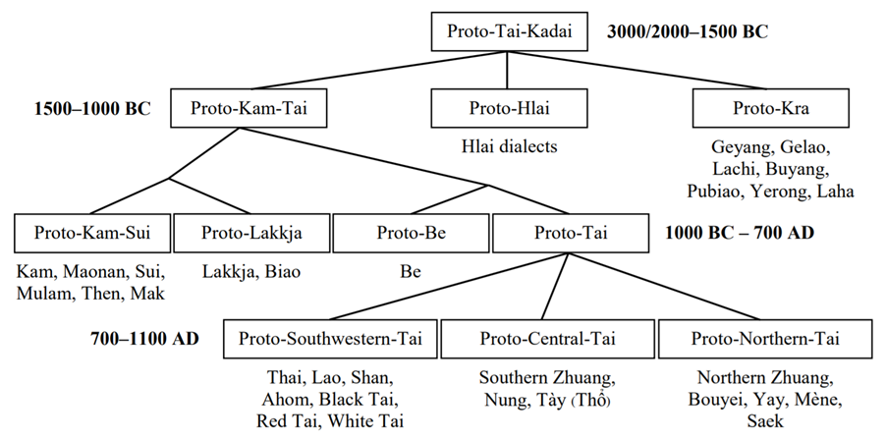
\includegraphics[width=\textwidth]{yurayong-img001.png}
% \begin{forest}for tree = {grow'=east, forked edges}
% [,phantom
%   [{3000/2000--1500 BC}, no edge
%     [{1500--1000 BC}, no edge
%       [{1000 BC -- 700 AD}, no edge, tier=tree_yurayong1
%         [{700--1100 AD}, no edge]
%       ]
%     ]
%   ]
% [Proto-Tai-Kadai,
%   [Proto-Kam-Tai,
%     [,shape=coordinate
%       [{Proto-Kam-Sui\\ \footnotesize Kam, Maonan, Sui,\\ \footnotesize Mulam, Them, Mak},tier=tree_yurayong1]
%       [{Proto-Lakkja\\ \footnotesize Lakkja, Biao}]
%     ]
%     [,shape=coordinate
%       [{Proto-Be\\ \footnotesize Be}]
%       [Proto-Tai
%         [{Proto-Southwestern-Tai\\ \footnotesize Tai, Lao, Shan,\\ \footnotesize Ahom, Black Tai,\\ \footnotesize Red Tai, White Tai}]
%         [Proto-Central-Tai]
%         [Proto-Northern-Tai]
%       ]
%     ]
%   ]
%   [{Proto-Hlai\\ \footnotesize Hlai dialects}]
%   [{Proto-Kra\\ \footnotesize Geyang, Gelao,\\ \footnotesize Lachi, Buyang,\\ \footnotesize Pubiao, Yerong, Laba}]
%  ]]
% \end{forest}
\begin{forest}
for tree = {
grow'=east,
forked edges,
anchor=west,
align=left
}
[,phantom
  [{3000/2000--\\1500 BC}, no edge, tier=tree_yurayong1
    [{1500--1000 BC}, no edge, tier=tree_yurayong2
      [{1000 BC -- 700 AD}, no edge, tier=tree_yurayong3
        [{700--1100 AD}, no edge, tier=tree_yurayong4]
      ]
    ]
  ]
[{Proto-\\Tai-Kadai},tier=tree_yurayong1
  [{Proto-\\Kam-Tai},tier=tree_yurayong2
    [,shape=coordinate
      [~\\Proto-Kam-Sui\\~,tier=tree_yurayong3,
        [{Kam, Maonan,\\ Sui, Mulam,\\ Then, Mak},tier=tree_nowadays]
      ]
      [{Proto-Lakkja},tier=tree_yurayong3
        [{Lakkja, Biao},tier=tree_nowadays]
      ]
    ]
    [,shape=coordinate
      [Proto-Be,tier=tree_yurayong3
        [Be,tier=tree_nowadays]
      ]
      [Proto-Tai,tier=tree_yurayong3
        [{Proto-\\Northern-Tai\\~},tier=tree_yurayong4
          [{Northern Zhuang,\\ Bouyei, Yay,\\ Mène, Saek},tier=tree_nowadays]
        ]
        [{Proto-\\Central-Tai},tier=tree_yurayong4
          [{Southern Zhuang,\\ Nung, Tày (Thổ)},tier=tree_nowadays]
        ]
        [{Proto-South\hyp \\western-Tai\\~},tier=tree_yurayong4
          [{Tai, Lao, Shan,\\Ahom, Black Tai,\\ Red Tai, White Tai},tier=tree_nowadays]
        ]
      ]
    ]
  ]
  [Proto-Hlai,tier=tree_yurayong2
    [Hlai dialects,tier=tree_nowadays]
  ]
  [Proto-Kra,tier=tree_yurayong2
    [{Geyang, Gelao,\\ Lachi, Buyang,\\ Pubiao, Yerong,\\ Laha},tier=tree_nowadays]
  ]
 ]
]
\end{forest}
\caption{\label{fig:yurayong:1}Diversification of Tai-Kadai languages (based on \citealt{Mitani1977}, \citealt{EdmondsonSolnit1997}, \citealt{Pittayaporn2014}).}
\end{figure}

As is indicated in \figref{fig:yurayong:1}, the Tai branch stems off from the Kam-Tai intermediate protolanguage, which makes the Kam-Sui languages linguistically closer to the Tai languages, compared to the more distantly related Kra and Hlai languages. This close genealogical tie is evident from a higher proportion of shared lexical items between Kam-Sui and Tai (see \citealt{Luo1988}, \citealt[4]{EdmondsonSolnit1997}).

In terms of geographical distribution, the Tai branch and its linguistic populations have spread out from their hypothetical Urheimat in South China towards South Asia and Mainland Southeast Asia. \figref{fig:yurayong:2} illustrates the speaking areas of modern Tai-Kadai languages. Today, there is a total of ca. 102 million Tai-Kadai speaking people \citep[199]{Liao2023a}, of which ca. 21 million are living in China. As can be seen from \figref{fig:yurayong:2}, the Tai branch has extended its speaking area to the south and west, significantly farther than its sister languages, Kam-Sui, Kra, and Hlai.

\begin{figure}
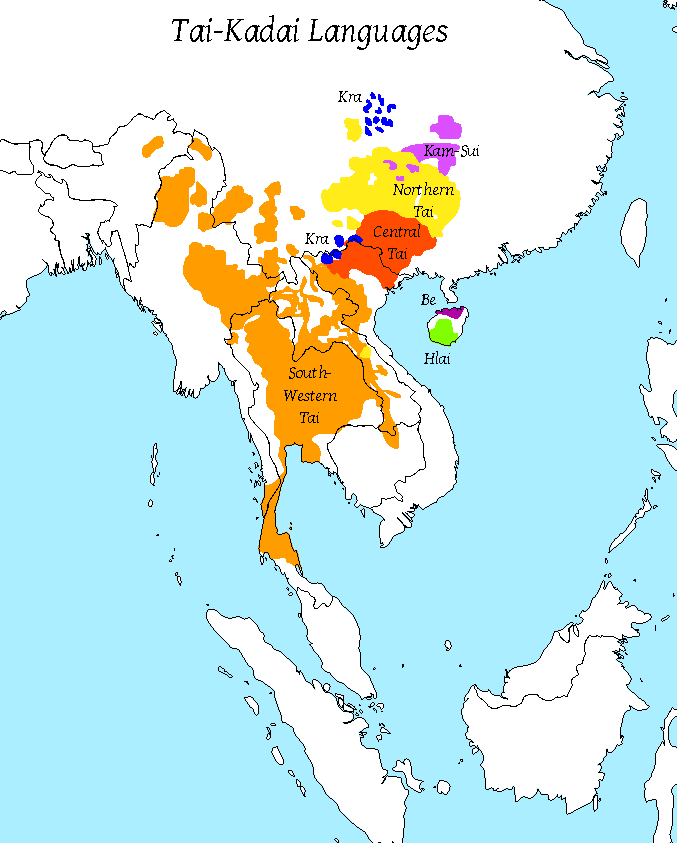
\includegraphics[width=\textwidth]{yurayong-img002.pdf}
\caption{\label{fig:yurayong:2}Geographical distribution of modern Tai-Kadai languages (public domain, \url{https://upload.wikimedia.org/wikipedia/commons/7/71/Taikadai-en.svg}).}
\end{figure}


Focusing on the Tai branch, previous studies have proposed a taxonomical structure with the following three major groups distributed across Mainland Southeast Asia (\citealt{Chamberlain1975}, \citealt{Li1977}; see also \citealt{Luo1997} for an alternative classification with four groups):

\begin{enumerate}
\item Northern Tai – the majority spoken in China, and the Saek language spoken in Laos, Thailand, and Vietnam
\item Central Tai – spoken in China and Vietnam
\item Southwestern Tai – spoken in China, India, Laos, Malaysia, Myanmar, Thailand, and Vietnam.
\end{enumerate}

In any case, such a subgrouping remains disputable when certain isoglosses concerning sound changes occur across subbranches. By only applying a conventional comparative method of historical linguistics, common patterns and clustering of phonological innovations namely do not give a straightforward dialectal classification. This is likely due to later language contact among Tai dialects, resulting from migration and relocation of the linguistic populations and causing convergence among Tai dialects spoken in adjacent areas (\citealt{Pittayaporn2009}, \citealt{Liao2023b}). A method which carefully deals with potential contact-induced changes and incorporates them into the classification yields a result illustrated in \figref{fig:yurayong:3}.

\begin{figure}
\footnotesize
% 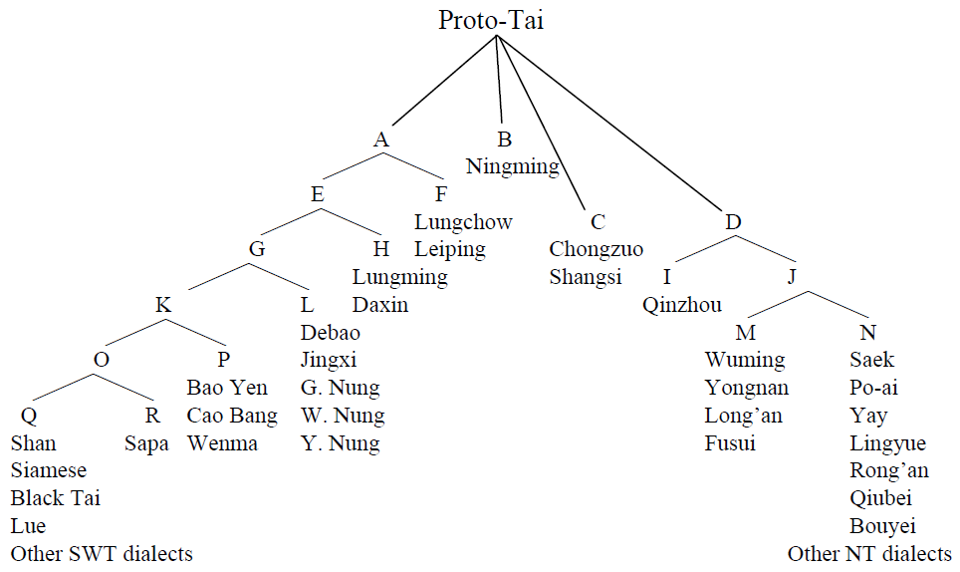
\includegraphics[width=\textwidth]{yurayong-img003.png}
\begin{forest}
for tree = {inner sep = 0cm, outer sep = 0cm, l sep = 1cm, s sep = 8pt}
[Proto-Tai
  [A
    [E
      [G
        [K
          [O
              [{Q\\Shan\\Siamese\\Black Tai\\Lue\\Other SWT\\dialects}]
            [{R\\Sapa}]
          ]
          [{P\\Bao Yen\\Cao Bang\\Wenma}]
        ]
        [{L\\Debao\\Jingxi\\G. Nung\\W. Nung\\Y Nung}]
      ]
      [{H\\Lungming\\Daxin}]
    ]
    [{F\\Lungchow\\Leiping}]
  ]
  [{B\\Ningming}]
  [{C\\Chongzuo\\Shangsi}]
  [D
    [{I\\Qinzhou}]
    [J
      [{M\\Wuming\\Yongnan\\Long'an\\Fusui}]
      [{N\\Saek\\Po-ai\\Yay\\Lingyue\\Rong'an\\Qiubei\\Buyei\\Other NT \\dialects}]
    ]
  ]
]
\end{forest}
\caption{\label{fig:yurayong:3} A classification of Tai dialects with reference to contact-induced changes \citep[298]{Pittayaporn2009}.}
\end{figure}

For instance, innovation Q concerns a sound change involving the merger \mbox{\textit{*kr-} = \textit{*ʰr-}}, which is the case in Shan, Thai (Siamese), Black Tai and Lue, but not in Sapa \citep[301]{Pittayaporn2009}.

In terms of population history, it has been the case especially in Laos and Thailand where people were compelled to migrate to new locations in the region, often as captives during the multiple war time periods between 1750 and 1850 \citep{Piyabhan1998}. The series of such historical events has given rise to new diaspora communities dispersing around Thailand in particular. The resettlement of Tai dialect speakers primarily concerned community members from the first generation, whereas the younger second and third generations of dialect speakers already exhibit signs of shifting towards a national language or the dominant regional dialect of their current location (\citealt{Akkharawatthanakun2003}, \citealt{BunyasathitEtAl2016}).

For many decades, the evolution and convergence among Tai dialects have been popular research topics in Thai and Tai-Kadai linguistics among researchers and students, particularly in Thai universities. Among hundreds of individual studies and theses published after the comprehensive handbook of Tai dialects by \citet{Li1977}, extensive works on Tai dialects by Gedney (edited by \citealt{Hudak2008}) and a comparative work on Tai tone paradigms by \citet{Brown1985}, there have been several large-scale comparative studies of tone paradigms. To name just few, the comparative approach has been applied for the investigation of tonal variation in Yo dialects \citep{Koowatthanasiri1981}, Phu Thai dialects \citep{Srithonrat1983}, Lao dialects \citep{Akkharawatthanakun2003}, Thai dialects in Malaysia \citep{Damanhuri2004}, Central Thai dialects \citep{Canilao2010}, Black Tai dialects \citep{Burusphat2012}, and Tai Lue dialects \citep{Akkharawatthanakun2020}. Consequently, the consensus is continuously evolving due to newly collected data from individual dialects which can contradict and deviate from earlier proposals in the genealogical classification of the Tai languages.

Participating in the ongoing discussion in dialectological studies of Tai-Kadai languages, our first goal in the present study is to identify change in progress. We choose homophones in tone paradigms of different Tai dialects as our object of study. The patterns of these homophones may have either resisted changes or diverged from their protosystems as we have arrived in the 21st century. Concretely, our attention is directed towards (i) paradigmatic tones DL and DS, which represent checked syllables with final stops [-p/-t/-k/-ʔ], and (ii) their alignment with tones A, B and C, which represent smooth syllables with final vowels or sonorants (see \sectref{sec:yurayong:2} for the detailed definition of tone paradigm).

The nature of the current study involves historical-comparative linguistics in conjunction with a quantitative approach, utilising computer-aided tools to investigate data from more than 300 different dialect speakers under investigation and aiming to trace significant signals of convergence among their tone paradigms. With this method, our second goal is to demonstrate how to address language changes occurring in the 21st century and their potential impact on how we read and interpret the taxonomical structure of the Tai languages.

We divide our study into five sections. After introducing the research questions, hypotheses, and historical background in \sectref{sec:yurayong:1}, in \sectref{sec:yurayong:2} we present a diachronic framework for the studies of tones, which has been previously employed for Tai as well as other Southeast Asian languages. Building upon the state of the art, in \sectref{sec:yurayong:3} we provide a description of how to apply a computer-aided quantitative method to investigate and analyse tone paradigm data from different Tai dialect speakers. Based on the data analysis, in \sectref{sec:yurayong:4} we discuss the scenarios of convergence and divergence of tone paradigms in general and in individual cases, which can be explained by sociolinguistic factors. Finally, in \sectref{sec:yurayong:5} we give some conclusional thoughts on the functionality of the applied quantitative method and highlight some areas which deserve attention in future studies and data collection, in order to conduct diachronic studies in an even more efficient manner.

\section{Tone system in Tai and other Southeast Asian languages}
\label{sec:yurayong:2}
Tones in Tai as well as in other languages in Southeast Asia, such as the cognate Kam-Sui, Hlai and Kra languages, along with neighbouring Chinese, Karenic, Hmong-Mien, and Vietic languages, are organised within a paradigm. A general principle dictates that the distribution of tones in paradigm is controlled by two factors: (i) the type of initial consonant, and (ii) the type of syllable. Both factors offer clues which can be traced back to phonological shapes at the protolanguage stage. Therefore, the tone paradigm serves as an important piece of evidence for reconstructing the lexicon of the protolanguage because sound changes, such as merger or loss of specific consonant types, may have left their traces on tones. This mechanism is called tonogenesis, which gave rise to tones as compensation for loss of certain phonetic features, most notably a voice distinction in the domain of consonants (see \citealt{Wulff1934}, \citealt{Haudricourt1954}, \citealt{Ferlus2004}, \citealt{Kingston2011}, \citealt{MichaudSands2020}). Naturally, this approach implies that the protolanguages did not originally possess tones, as has been discussed, most notably, for Chinese (\cites[593]{Handel2014}[182]{Hill2019}).

In the case of Tai languages, a classification of four types of initial consonants has been associated with different pitch patterns as given below (see e.g. \citealt{Maddieson1984} and \citealt{Ratliff2015} for the effect of voicing in pitch). One of the common practices to annotate pitches and contours in the studies of East Asian linguistics uses numbers to indicate pitch height: 1 = lowest pitch vs. 5 = highest pitch.

\begin{enumerate}
\item Aspirated – high pitch
\item Voiceless – mid pitch
\item Implosive – mid pitch
\item Voiced – low pitch
\end{enumerate}

Note that the relation between manner of articulation and pitch presented here should not be taken as an absolute linguistic universal. Some Tai-Kadai languages, namely, exhibit no significant correlation between aspiration and high pitch (see \cites[38]{Zhang1980}[188]{Edmondson1990}[170--171]{Liao2016}[18]{ZhuEtAl2016}). Furthermore, the status of the aspirated initials remains a subject of dispute, with questions surrounding whether they can be reconstructed as far as to Proto-Tai or only to the Proto-Southwestern-Tai intermediate stage (see arguments in \citealt{LiangZhang1996}, \citealt{Pittayaporn2009}, with a summary provided in \citealt{Liao2023a}). Another dimension to consider is the syllable type, which leads to a division of four tone classes, a.k.a. tonal splits: A, B, C (smooth syllables ending with vowels or sonorants), and DL, DS (checked syllables ending with stops [-p/-t/-k/-ʔ]).

The two factors discussed above serve as the foundation for the tool known as ``Gedney’s tone box" (see \tabref{tab:yurayong:1}), which was initially proposed by William J. \citet{Gedney1972} and is recognised as one of the main comparative tools in the Tai-Kadai linguistics scholarship. Based on the original tone box by Gedney, we have systematised and relabelled the tone slots for the comparative purpose of the present study (see \tabref{tab:yurayong:2}). According to \citet[271]{Pittayaporn2009}, contour characteristics of each tone are reconstructed for Proto-Tai as follows: A~= mid-level, B~= low-rising, C~= high-falling, and D~= low-rising. 

\begin{table}
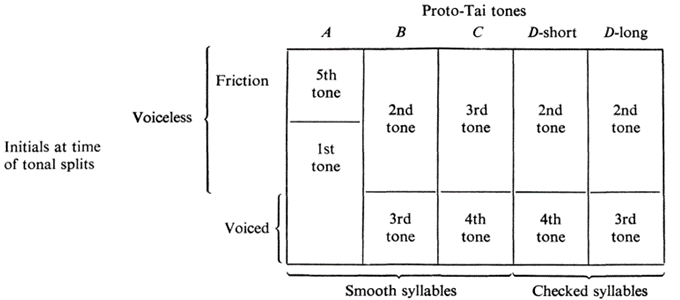
\includegraphics[width=\textwidth]{yurayong-tab001.png}
\caption{The original \citegen{Gedney1972} Tai tone box for Proto-Tai}
\label{tab:yurayong:1}
\end{table}

\begin{table}
\begin{tabular}{l *5{c} }
\lsptoprule
Initial consonant class & \\
at time of tonal splits & A & B & C & DL(ong) & DS(hort)\\\midrule
Aspirated & A1 & B1 & C1 & DL1 & DS1\\
Plain & A2 & B2 & C2 & DL2 & DS2\\
Implosive & A3 & B3 & C3 & DL3 & DS3\\
Voiced & A4 & B4 & C4 & DL4 & DS4\\
\lspbottomrule
\end{tabular}
\caption{The modified Tai tone box (based on \citealt{Gedney1972}).}
\label{tab:yurayong:2}
\end{table}

In any case, it is important to note that Gedney’s tone box has been primarily developed within the context of the Southwestern branch of Tai languages. Consequently, it often has issues when applied to explain the tone paradigms in other subbranches, i.e. Central and Northern Tai, not to mention the more distantly related Tai-Kadai languages like Kam-Sui, Kra and Hlai (see the criticisms on cross-family validity of Gedney’s tone box tool in \citealt{Liao2023a}).

A similar type of tone box is also employed in the studies of tones in Chinese, Karenic, Hmongic and Vietic languages. However, some languages may distinguish only a contrast between voiceless and voiced initial stops, while the aspirated and implosive classes are grouped within the same category as voiceless stops, making only the voice distinction between the initial consonant classes. Similarly, the vowel length distinction is not considered a meaningful category in some languages. See, for instance, a tone box with only two initial consonant classes, based on the reconstructed Middle Chinese tone paradigm and used to describe tone paradigms across modern Chinese dialects in \tabref{tab:yurayong:3}. Interestingly, certain Middle Chinese tone names appear to record the contour characteristics pronounced during the Middle Chinese period (cf. the reconstruction of Proto-Tai tone contours in \citealt[271]{Pittayaporn2009}).


\begin{table}
\begin{tabular}{l *4{c} }
\lsptoprule
    & \multicolumn{4}{c}{Middle Chinese name of tone}\\\cmidrule(lr){2-5}
    & {\ChineseFandolSong 平} \textit{píng}    & {\ChineseFandolSong 上} \textit{shǎng}   & {\ChineseFandolSong 去} \textit{qù}  & {\ChineseFandolSong 入} \textit{rù} \\
    & {‘level’} & {‘rising’} & {‘falling’} & {‘entering’}\\
\midrule
Tone label         & A\phantom{1} & B\phantom{1} & C\phantom{1} & D\phantom{1}\\
Voiceless initials & A1 & B1 & C1 & D1\\
Voiced initials    & A2 & B2 & C2 & D2\\
\lspbottomrule
\end{tabular}
\caption{The Chinese tone box\label{tab:yurayong:3}}
\end{table}


From the paradigms in modern Tai languages, we know that tone D can be traced back to a checked syllable structure ending with stops [-p/-t/-k] in Proto-Tai. However, there is unfortunately no internal evidence available for syllable structures of tones A, B and C prior to the emergence of tones in Proto-Tai-Kadai. This is in contrast to some other neighbouring languages, for example, Chinese where sufficient evidence for syllable structures during the pre-tonal Old Chinese stage is attested in earlier written sources and phonological adaptation of Sanskrit loanwords in Old Chinese, as well as Old Chinese loanwords in Korean (\cites[594]{Handel2014}[184--185]{Hill2019}). A reconstruction of the Old Chinese syllable structures is given as follows:

\begin{enumerate}
\item A – a syllable ending with a vowel or sonorant
\item B – a syllable ending with a glottal stop [-ʔ]
\item C – a syllable ending with a sibilant [-s]
\item D – a syllable ending with a stop [-p/-t/-k]
\end{enumerate}

Similar patterns and mechanisms have also been applied together with evidence from Chinese loanwords to explain tonogenesis in Hmong-Mien \citep[183--184]{Ratliff2010} and Vietic \citep{Thurgood2002}, both of which have undergone early contact with Chinese. Interestingly, in the field of Tai-Kadai linguistics, there has been no serious attempt to reconstruct distinct original syllable types for tones A, B and C in Proto-Tai-Kadai and their corresponding reflexes in subsequent intermediate protolanguages, although there are ample early Chinese loanwords available for similar analysis (cf. \citealt{Pittayaporn2014}), as has been done for Hmong-Mien and Vietic.

Relevant to the current study which focuses on Tai tone paradigms is the observation that tones DL and DS always align paradigmatically with some of the twelve phonemic tone slots in columns A, B, and C (cf. the similar low-rising contour reconstructed for tones B and D as given in \citealt[271]{Pittayaporn2009}). However, in practice, the maximum number of phonemic tone distinctions observed in Tai-Kadai languages is nine, often due to the merger of tones between the plain (tones A2/B2/C2/D2) and implosive (tones A3/B3/C3/D3) classes of initial consonants in most languages. Ultimately, only a few Tai-Kadai languages possess nine distinct phonemic tones in a symmetrical fashion, a characteristic primarily found in certain dialects of the Kam language within the Kam-Sui branch. \tabref{tab:yurayong:4} illustrates pairs of examples, where the former represents a smooth syllable (tone A, B, or C) and the latter represents a checked syllable (tone DL or DS), except the last three tones (53, 453, and 33) which only occur in smooth syllable.
Despite the symmetrical case of three consonant classes combined with three syllable types in Kam, the average number of tones across the Tai-Kadai family typically falls within the range of five to seven tones (see e.g. \citealt{Brown1985}, \citealt{Hudak2008}).

\vfill
\begin{table}[H]
\small
\begin{tabular}{rll}
\lsptoprule
  Tone value & Example & Gloss\\
  (contour) & & \\
  \midrule
 55 & \textit{ma}\textsuperscript{55} & ‘vegetable’\\
    & \textit{jɑk}\textsuperscript{55} & ‘wet’\\
 35 & \textit{ma}\textsuperscript{35} & ‘to come’\\
    & \textit{mat}\textsuperscript{35} & ‘flea’\\
 11 & \textit{ma}\textsuperscript{11} & ‘tongue’\\
    & \textit{sɑk}\textsuperscript{11} & ‘thief’\\
323 & \textit{ma}\textsuperscript{323} & ‘cloud, soft’\\
    & \textit{mak}\textsuperscript{323} & ‘big’\\
\lspbottomrule
\end{tabular}
\begin{tabular}{rll}
\lsptoprule
  Tone value & Example & Gloss\\
   (contour) & & \\
  \midrule
 13 & \textit{no}\textsuperscript{13} & ‘rat’\\
    & \textit{pʰat}\textsuperscript{13} & ‘blood’\\
 31 & \textit{ma}\textsuperscript{31} & ‘horse’\\
    & \textit{mak}\textsuperscript{31} & ‘ink’\\
 53 & \textit{ja}\textsuperscript{53} & ‘paddy, wet field’\\
453 & \textit{ma}\textsuperscript{453} & ‘to soak (rice)’\\
 33 & \textit{pa}\textsuperscript{33} & ‘rice husk’\\
 & & \\
\lspbottomrule
\end{tabular}
\caption{Tones of common Kam (modified from \citealt[514]{YangEdmondson2008}).}
\label{tab:yurayong:4}
\end{table}
\vfill\pagebreak


The subgrouping of individual Tai languages can be discerned through both consonant and vowel inventories, as well as their tone paradigm. Concerning the latter, the distinctive homophone patterns across tone slots exhibit characteristics specific to individual language groups. This aspect of tone paradigms has significantly received scholarly attention within the field of Tai dialectology (see e.g. \citealt{Brown1985}, \citealt{Dockum2019}). Below, we present several characteristics unique to individual dialects, which are not commonly observed in other dialectal groups. These examples are drawn from dialectal data in \citet{Brown1985} and \citet{Hartmann2008} and specifically focus on the fundamental paradigmatic tones A, B, and C. Further explanations regarding individual dialectal groups are provided below following the paradigmatic summary in \tabref{tab:yurayong:5}.
\largerpage[-2]


\begin{table}
% \begin{tabular}{ *{11}{c} }
% \lsptoprule
% \multicolumn{3}{c}{{Tai Lue \&}} & {} & \multicolumn{3}{c}{{Tai Yuan/}} & \\
% \multicolumn{3}{c}{{White Tai}}  & {} & \multicolumn{3}{c}{{Northern Thai}} & & \multicolumn{3}{c}{{Lao}}\\\cmidrule(lr){1-3}\cmidrule(lr){5-7}\cmidrule(lr){9-11}
% {A1} & B1 & C1 &  & A1 & {B1} & {C1} &  & {A1} & {B1} & C1\\
% {A2} & B2 & C2 &  & A2 & {B2} & {C2} &  & {A2} & {B2} & C2\\
% {A3} & B3 & C3 &  & A3 & {B3} & {C3} &  & {A3} & {B3} & C3\\
% {A4} & B4 & C4 &  & A4 & {B4} & {C4} &  & {A4} & {B4} & C4\\
% \midrule
% \multicolumn{3}{c}{{Shan \& }} & \\
% \multicolumn{3}{c}{{Central Thai}} & {} & \multicolumn{3}{c}{{Southern Thai}} &  &  & \\\cmidrule(lr){1-3}\cmidrule(lr){5-7}
% A1 & B1 & C1 &  & A1 & B1 & C1 &  &  &  & \\
% A2 & B2 & C2 &  & A2 & B2 & C2 &  &  &  & \\
% A3 & B3 & %%[Warning: Draw object ignored]
% C3 &  & A3 & B3 & C3 &  &  &  & \\
% {A4} & B4 & {C4} &  & A4 & {B4} & {C4} &  &  &  & \\
% \lspbottomrule
% \end{tabular}
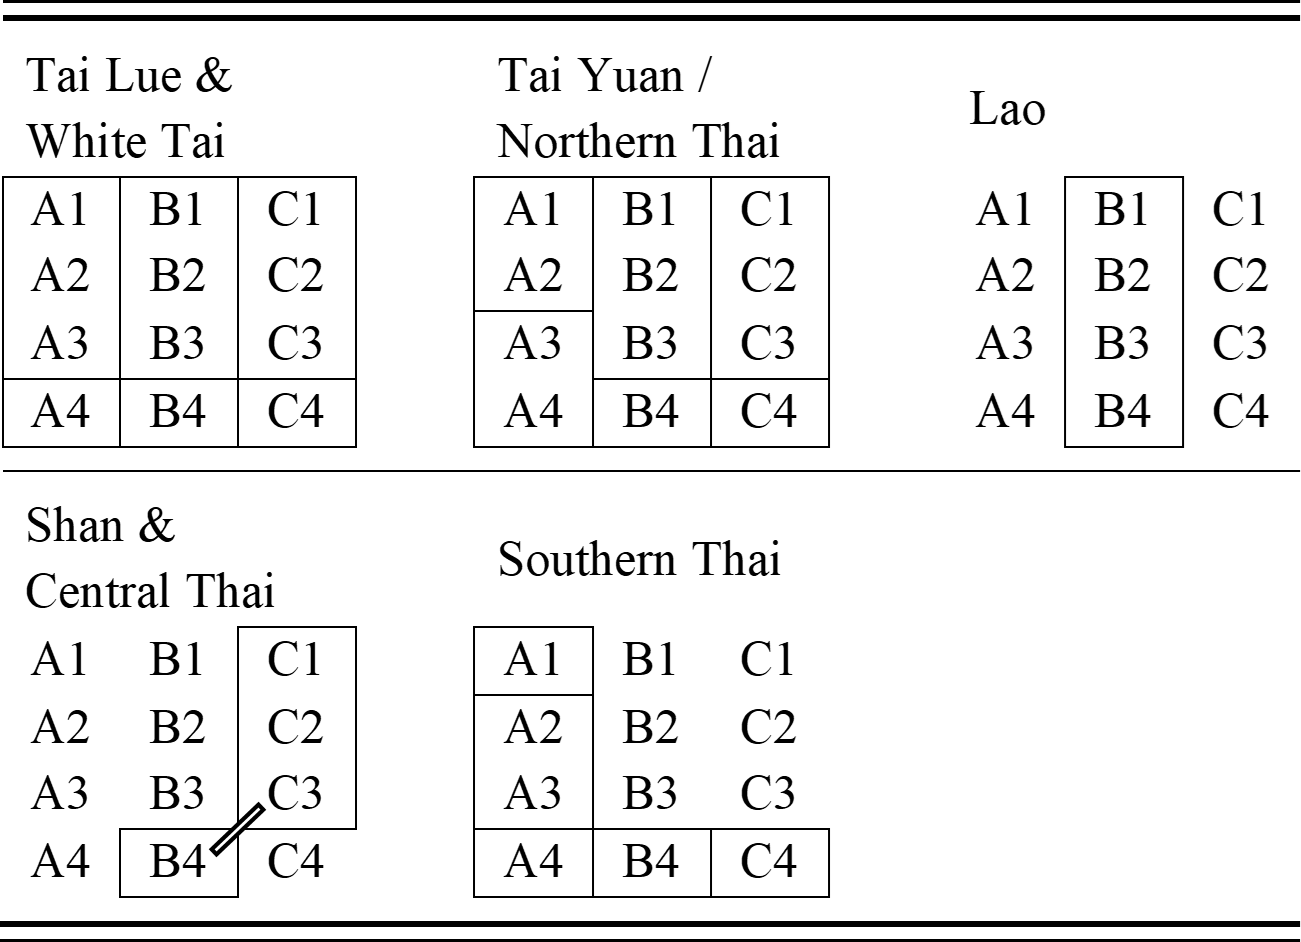
\includegraphics[scale=.8]{20240810 grafiken yurayong neu/Table 5_new.png}
\caption{Some characteristics of the tone paradigms in the selected Tai dialectal groups.}
\label{tab:yurayong:5}
\end{table}

\begin{enumerate}
\item Tai Lue and White Tai dialects – a symmetrical split of all the paradigmatic tones A, B and C for smooth syllables between the original unvoiced and voiced initials
      \begin{itemize}[label=→]
        \item A1, A2, A3 ${\neq}$ A4
        \item B1, B2, B3 ${\neq}$ B4
        \item C1, C2, C3 ${\neq}$ C4
      \end{itemize}
  
\item Tai Yuan\slash Northern Thai dialects – a symmetrical split as observed in Tai Lue dialects, but with a distinction between the original aspirated/plain and implosive/voiced initials within the paradigmatic tone A
      \begin{itemize}[label=→]
        \item A1, A2 ${\neq}$ A3, A4
        \item B1, B2, B3 ${\neq}$ B4
        \item C1, C2, C3 ${\neq}$ C4
      \end{itemize}
      
\item Lao dialects – a merger of all tone slots within the paradigmatic tone B
      \begin{itemize}[label=→]
        \item B1 = B2 = B3 = B4
      \end{itemize}

\item Shan and Central Thai dialects – a diagonal alignment of the original aspirated/plain/implosive and voiced initials within paradigmatic tones B and C
      \begin{itemize}[label=→]
        \item  C1, C2, C3 = B4
      \end{itemize}

\item Southern Thai dialects – a symmetrical split of the paradigmatic tones within tone A with distinctions for the original aspirated, plain/implosive and voiced initials, as well as a symmetrical split of the paradigmatic tones A, B, and C with the original voiced initials
      \begin{itemize}[label=→]
        \item A1 ${\neq}$ A2, A3 ${\neq}$ A4
        \item A4 ${\neq}$ B4 ${\neq}$ C4
      \end{itemize}
\end{enumerate}

Next, we shift our focus to the primary data of the present study and the computer-aided methods and processes employed therein.

\section{Data and methods}
\label{sec:yurayong:3}
\subsection{Data coverage}
\label{sec:yurayong:3.1}
In the present study, we conduct a comprehensive investigation using 315 datapoints obtained from data of speakers of Tai dialects, primarily from regions outside China. Our focus is on analysing patterns observed within the tone paradigm. The data is collected from a range of grammatical and phonological descriptions of Tai dialects in Mainland Southeast Asia. These descriptions have been published during the late-20th and early-21st centuries. Most, if not all, of the sources provide empirical data of individual dialect speakers, presented in the form of word lists covering all the tone slots outlined in \tabref{tab:yurayong:2}. Alignment patterns observed among different tone slots are also often discussed in a tone box similar to that of \tabref{tab:yurayong:5}. The majority of these sources usually have their goal in describing how the observed tone paradigms correspond to or deviate from the common pattern of the specific Tai language. Some works, most notably \citet{Akkharawatthanakun2003}, further delve into sociolinguistic factors which may have significantly influenced the evolution of the tone paradigm when such data is available and feasible from speech communities (see \sectref{sec:yurayong:4} for a similar attempt in the present study).

Out of the 315 datapoints, the data covers dialects from a total of 17 different Tai languages as listed below.\footnote{The full details and sources for each datapoint can be found in the supplementary material: \url{https://researchportal.helsinki.fi/files/244396698/Convergence_and_divergence_of_tone_paradigms_across_Tai_dialects_in_the_21st_century_supplementum_.xlsx}.}

\begin{multicols}{2}
\begin{enumerate}
\item Tai Lue                          
\item Tai Yuan\slash Northern Thai         
\item Phu Thai                         
\item Northern Lao (Luang Phrabang)    
\item Central Lao (Vientiane)          
\item Southern Lao (Champasak)         
\item Western Lao\slash Northeastern Thai  
\item Central Thai                      
\item Southern Thai 
\item Saek
\item Shan
\item White Tai
\item Black Tai
\item Yo
\item Yoy
\item Phuan
\item Khorat Thai
\end{enumerate}
\end{multicols}

In the 21st century, dialects of various languages are spoken in diaspora areas, particularly among Lao dialect speakers who have relocated from the dialectal core regions in Luang Phrabang, Vientiane, or Champasak to various areas of Thailand. The geographic locations of the speakers included in the dataset are cartographically illustrated in \figref{fig:yurayong:4}, using ArcGIS tools. As can be seen from the map in \figref{fig:yurayong:4}, a noteworthy proportion of dialect speakers are not located within the core area of their respective languages, particularly the Lao diaspora dialects due to their migration history discussed by Piyabhan (\citeyear{Piyabhan1998}, mentioned in \sectref{sec:yurayong:1}). This phenomenon raises an important issue potentially contributing to the restructuring of tone paradigms among certain dialect speakers, a matter which will be discussed further in \sectref{sec:yurayong:4}.


\begin{figure}    
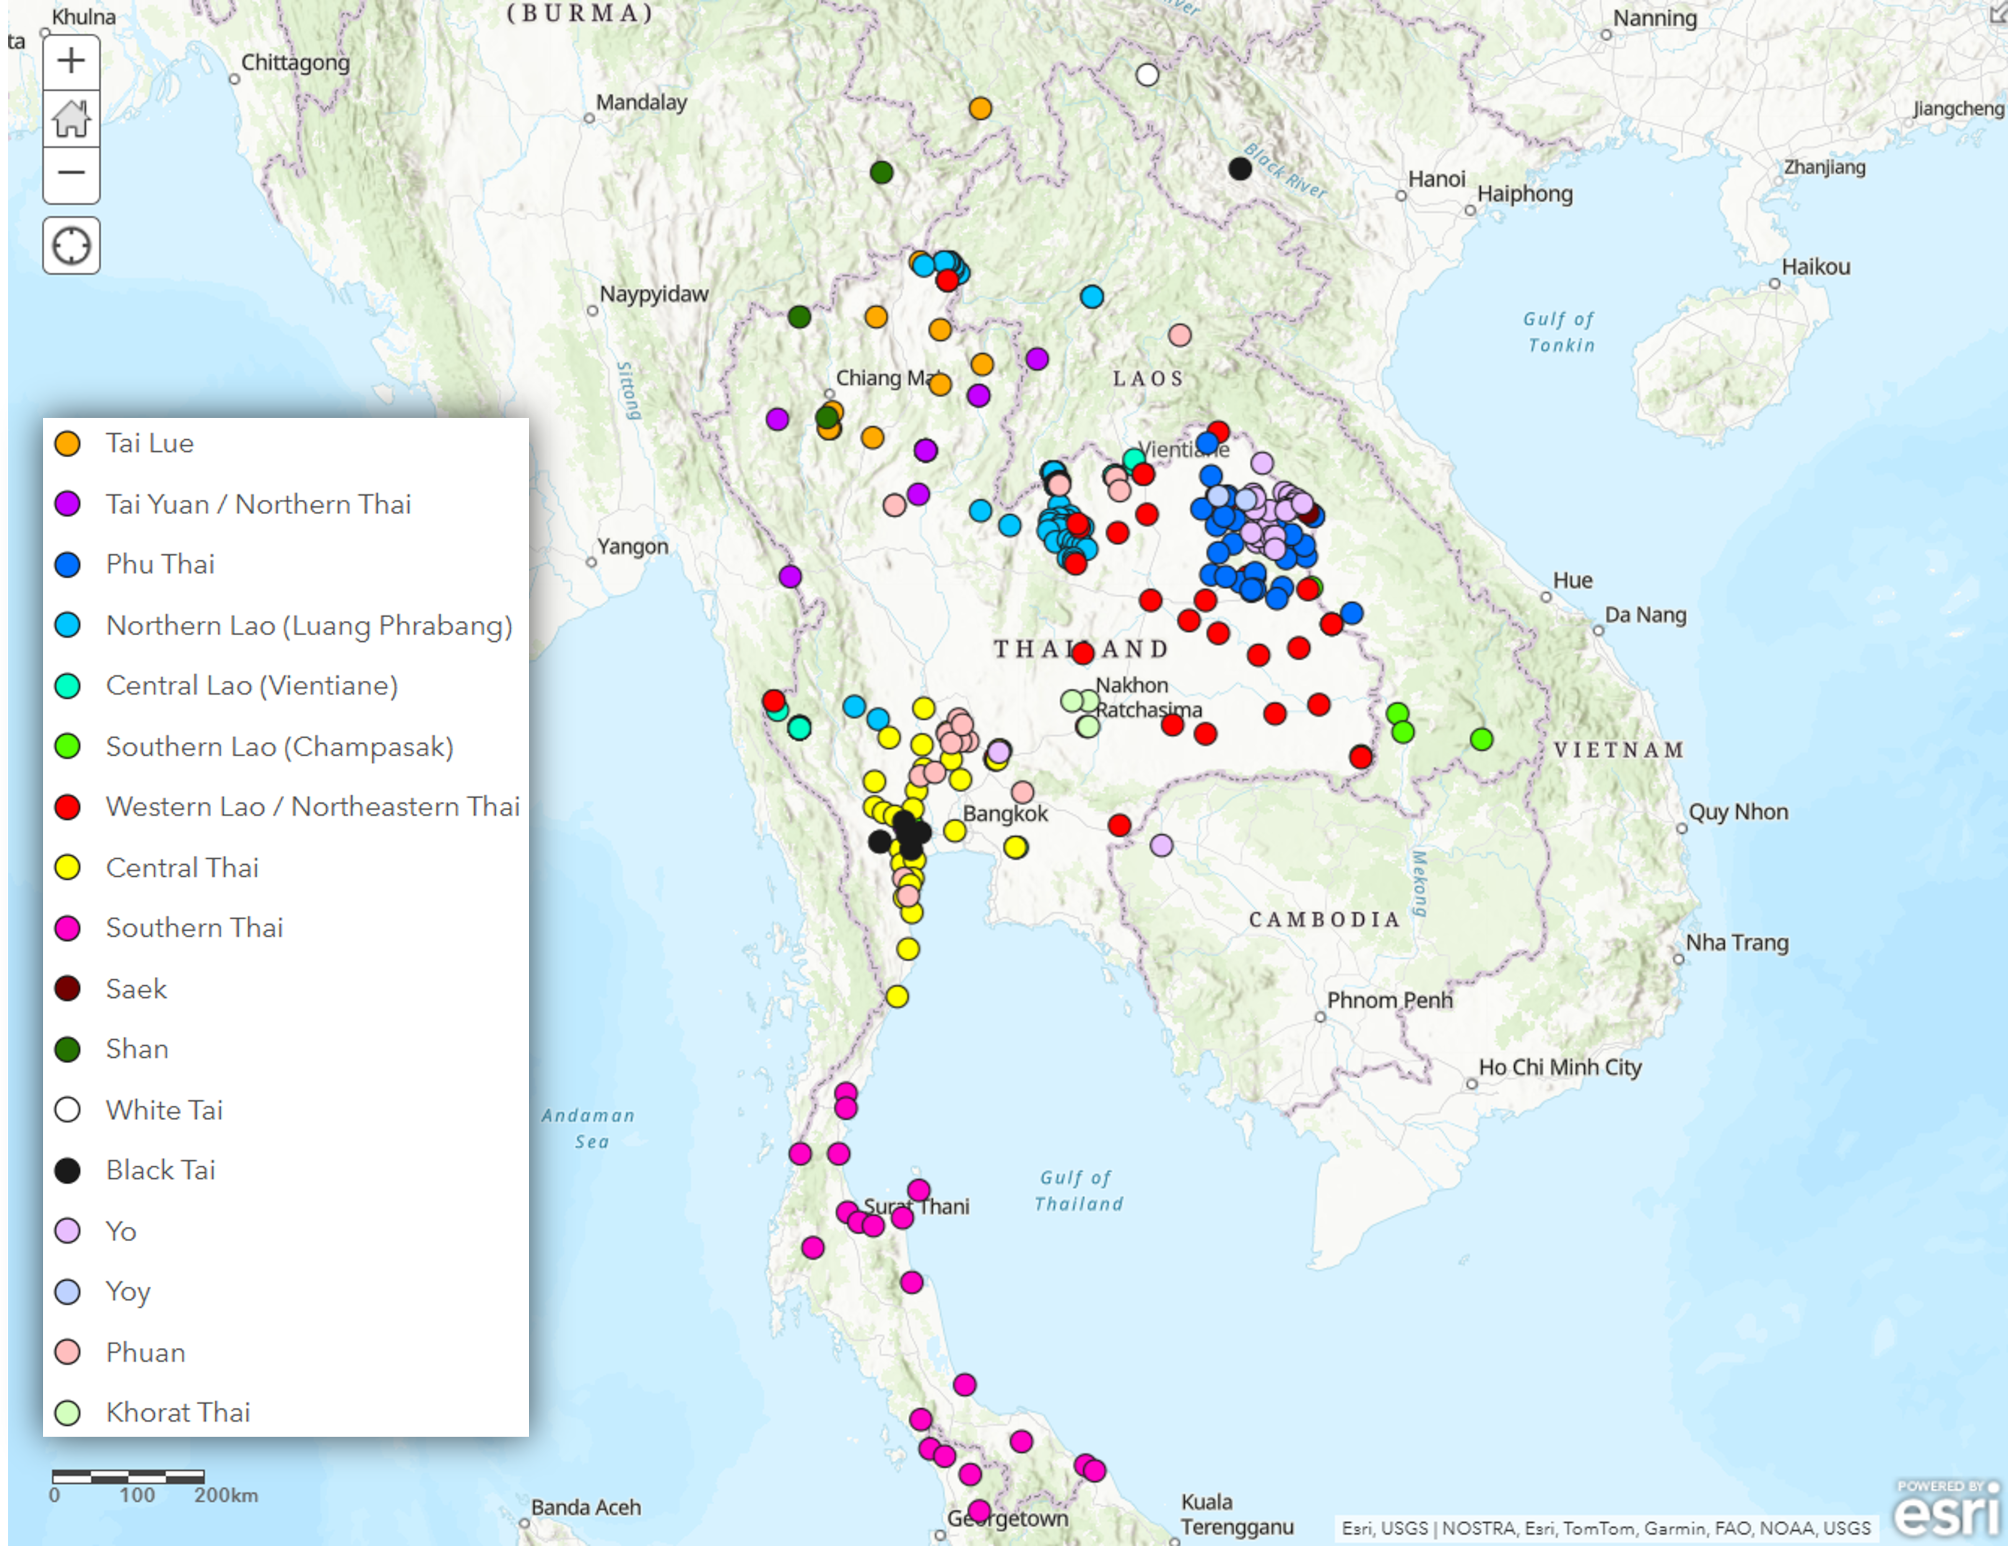
\includegraphics[width=\textwidth]{Figure4.png}
\caption{\label{fig:yurayong:4}Datapoints of the Tai dialect speakers under investigation.}
\end{figure}


\subsection{Methods for data illustration and analysis}
\label{sec:yurayong:3.2}
As a general principle for organising the data, the information collected from various grammatical and phonological descriptions of Tai dialects is arranged based on whether tones DL and DS align with tones A, B, and/or C within individual dialects. This compiled information is then processed by a Neighbor-Net algorithm \citep{BryantMoulton2004}. The outcome of this processing is a network diagram visualising the clustering and distances among typological profiles of each dialect under investigation. Importantly, this diagram is generated without exhibiting any bias towards the genealogical relationship or distances across dialects. This approach has been effectively applied to studies of several language families across Eurasia (e.g. \citealt{GrünthalNichols2016}, \citealt{SzetoEtAl2018}, \citealt{Nichols2020}, \citealt{YurayongSzeto2020}, \citealt{SzetoYurayong2021}). The data processing involves four different steps, which are elaborated upon in the following points below.

\subsubsection{Step 1: From language description to tone paradigm}\label{sec:yurayong:3.2.1}

It is a common practice in Tai-Kadai linguistics for the phonological descriptions of Tai dialects to include details about tone contours (1 = lowest pitch vs. 5 = highest pitch) and paradigms presented in the form of tone box (as previously illustrated in \tabref{tab:yurayong:2} within \sectref{sec:yurayong:2}). Utilising these tone boxes, the homophones between paradigmatic tones DL and DS, juxtaposed with tones A, B, and C, can be identified, as exemplified in \tabref{tab:yurayong:6}. The tone paradigm in \tabref{tab:yurayong:6} reveals that the speaker of the Central Lao dialect spoken in Suan Pan, Nakhon Pathom province of Thailand, has six distinct phonemic tones. Among these, four alignment patterns of tones DL and DS are identified: (i) DL123 = C1, (ii) DL4 = C234, (iii) DS123 = A1, and (iv) DS4 = B1234. The alignment patterns, identified from the tone paradigms of individual dialect speakers, serve as the focal points of comparison in the quantitative analysis conducted in the present study.

\begin{table}
% \begin{tabular}{l *6{c} r@{~}c@{~}l }
% \lsptoprule
% Initial consonant class & \\
% at time of tonal splits & A & B & C & DL & DS & → & \multicolumn{3}{c}{Alignment pattern}\\\midrule
% Aspirated & 24 & 33 & 21 & 21 & 24 &  & DL123  & = & C1\\
% Plain & 232 &  &  &  &  &             & DL4    & = & C234\\
% Implosive &  &  &  &  &  &            & DS123  & = & A1\\
% Voiced & 353 &  & 41 & 41 & 33 &      & DS4    & = & B1234\\
% \lspbottomrule
% \end{tabular}
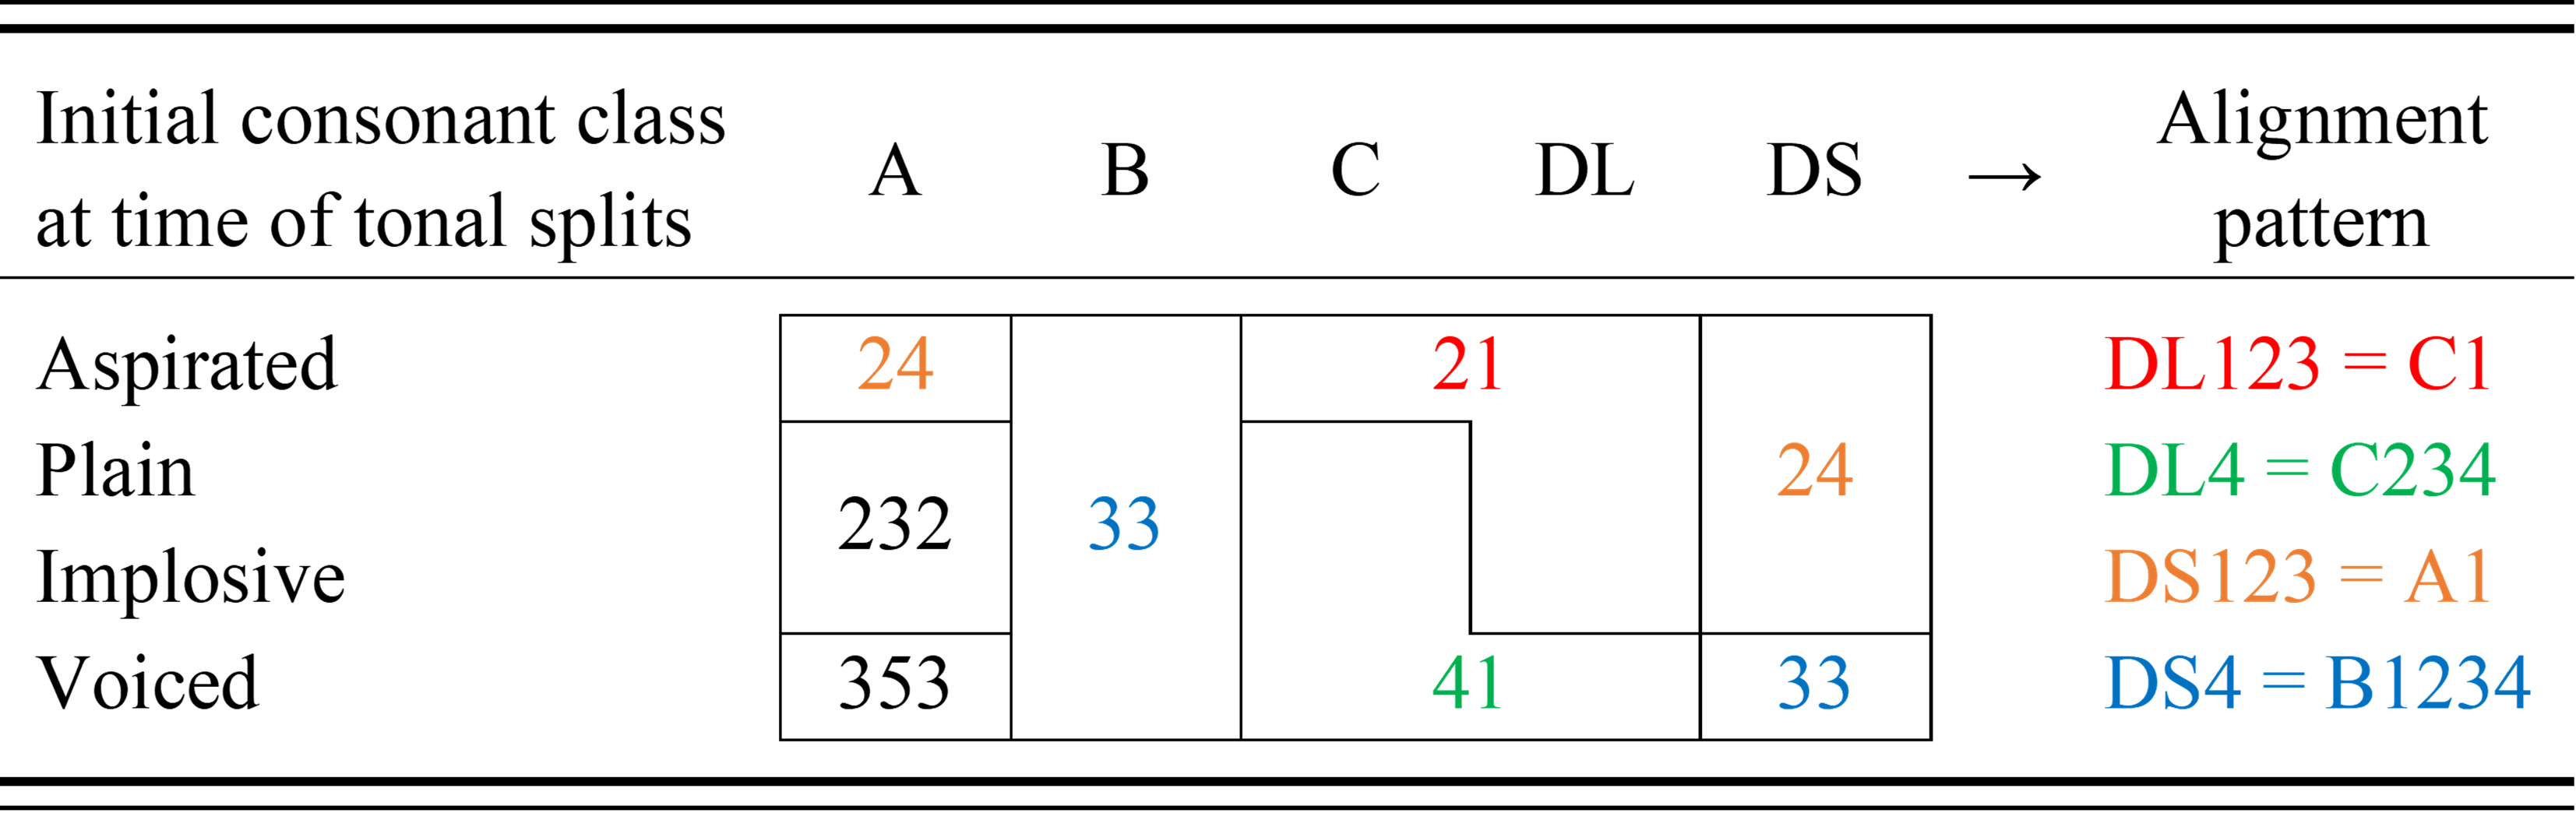
\includegraphics[width=\textwidth]{20240810 grafiken yurayong neu/Table 6.png}
\caption{The tone paradigm of the Central Lao dialect speaker (LC24) in Suan Pan, Nakhon Pathom province, Thailand.}
\label{tab:yurayong:6}
\end{table}



\subsubsection{Step 2: From tone paradigm to binary data}
\label{sec:yurayong:3.2.2}
The homophones aligned between tones DL and DS and tones A, B, and C are then converted into binary values: 0 = no alignment vs. 1 = alignment present, as displayed in \tabref{tab:yurayong:7}. This binary value representation characterises the tonological profile of each dialect speaker, drawing an analogy to chromosomes and their sequencing within a species. This is a concept commonly employed in evolutionary studies, in which the original development of this method finds its root (see general principles for the application of Neighbor-Net diagrams in evolutionary studies in \citealt{MaddisonEtAl1997}, \citealt{HusonBryant2006}). Subsequently, this dataset of tonological profiles will serve as a foundational component for data illustration model generated by the Neighbor-Net algorithm in Step 4 described in \sectref{sec:yurayong:3.2.4}.

\begin{table}
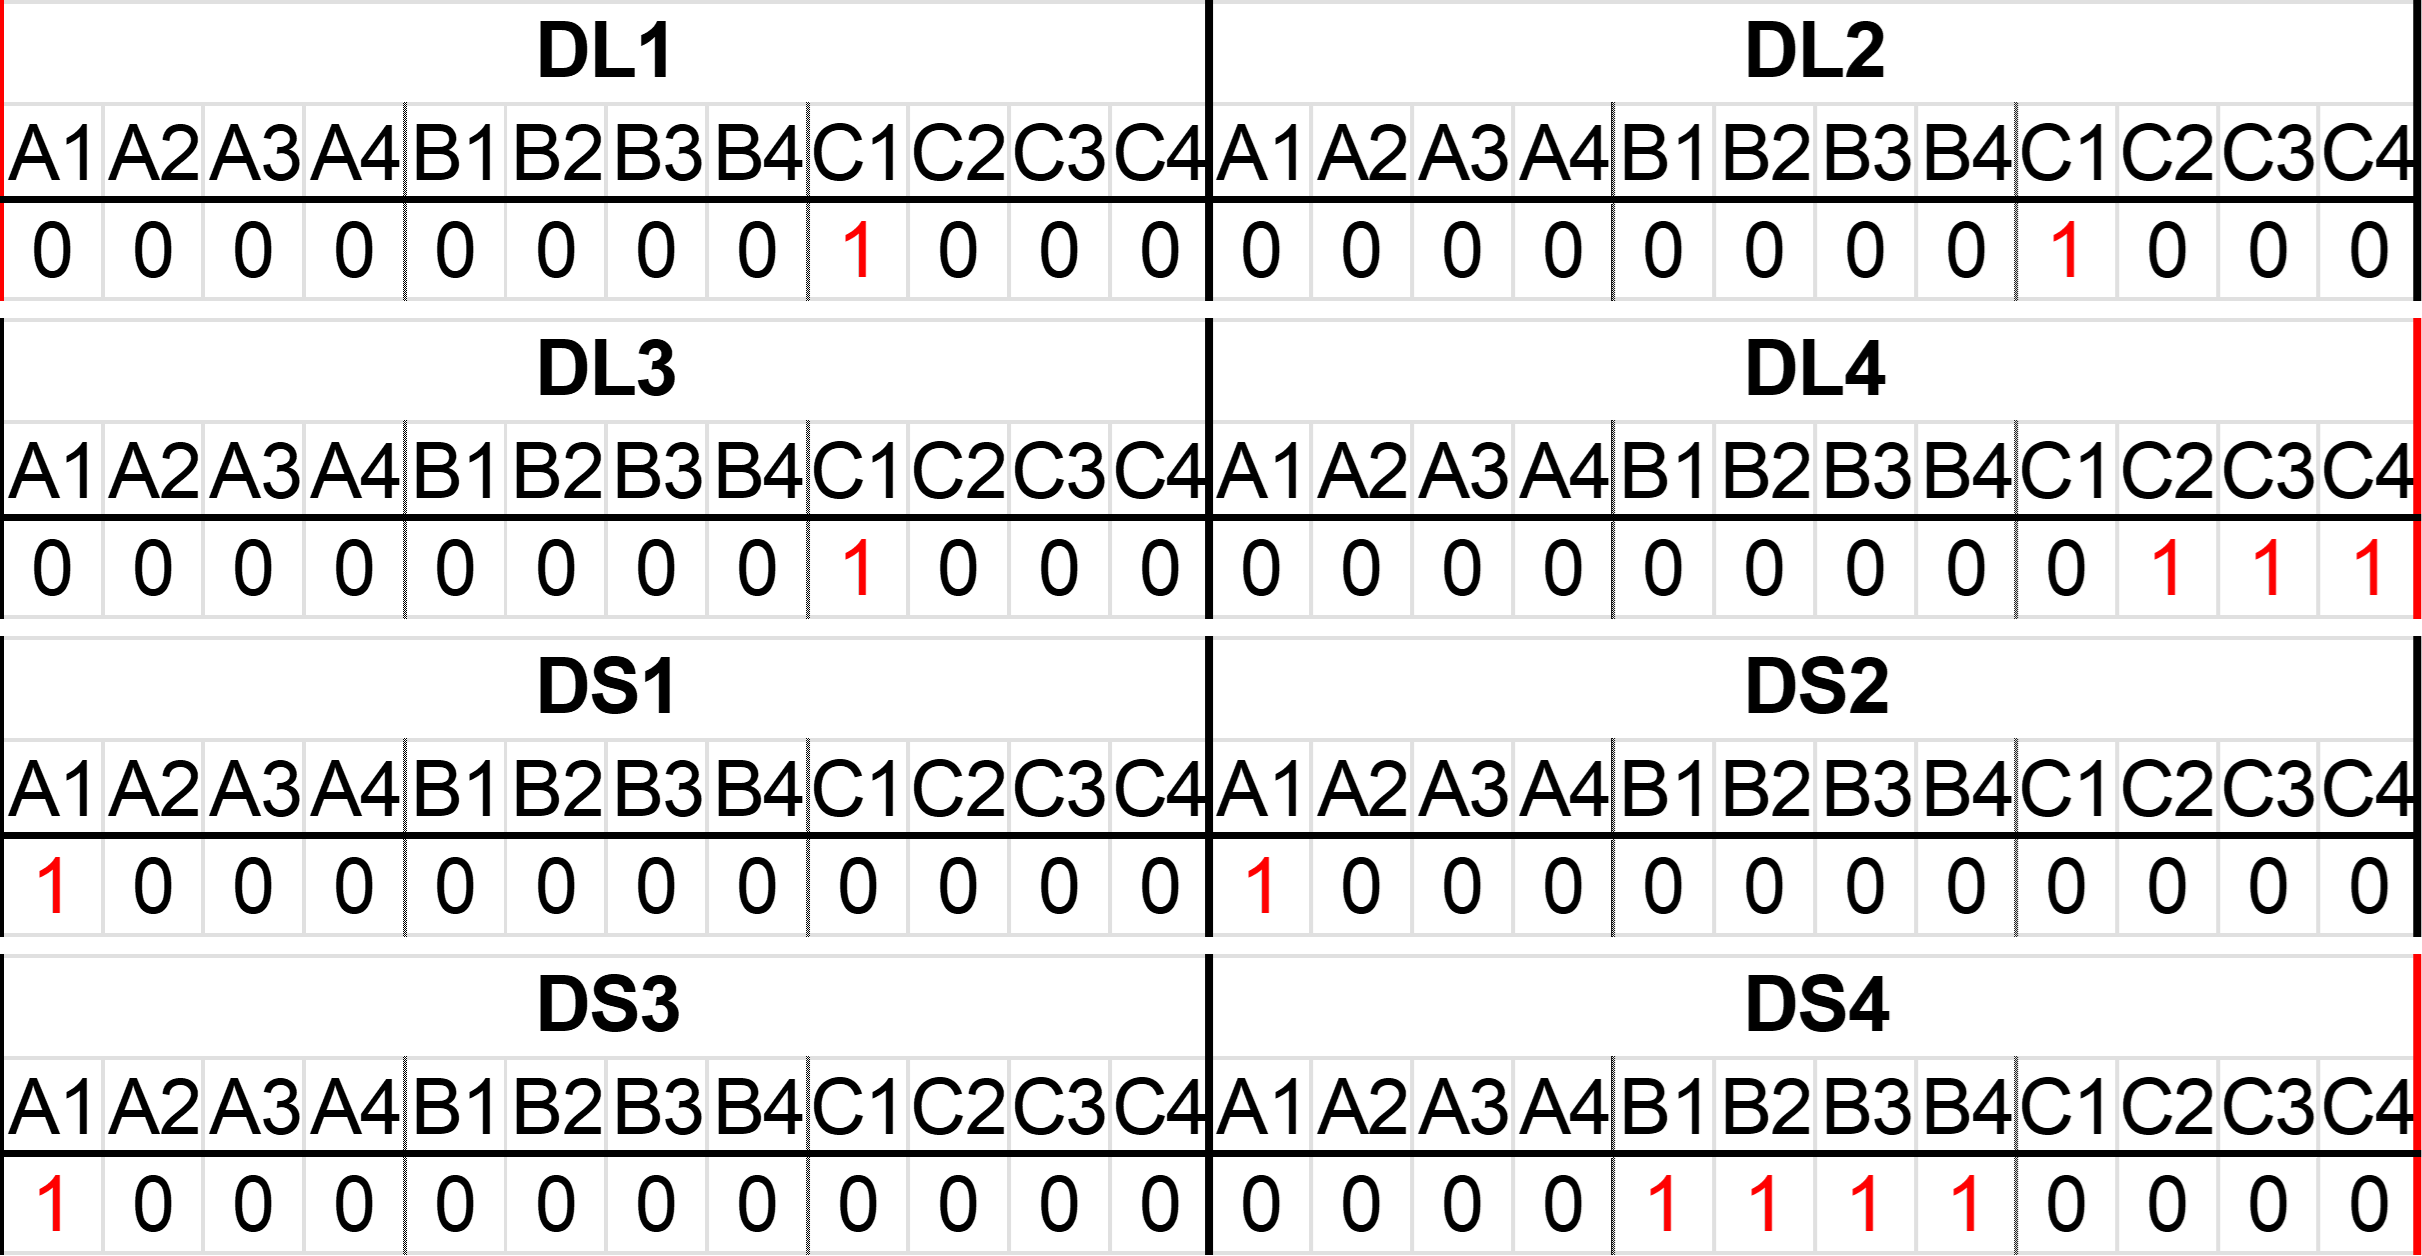
\includegraphics[width=\textwidth]{yurayong-tab002.png}
\caption{The tonological profile of the Central Lao dialect speaker (LC24) in Suan Pan, Nakhon Pathom province, Thailand.}
\label{tab:yurayong:7}
\end{table}


\subsubsection{Step 3: From binary data to nexus format}
\label{sec:yurayong:3.2.3}
The binary data is converted into the nexus format \citep{MaddisonEtAl1997} which is a kind of structured and systematic data format for facilitating computational modelling tasks, such as the implementation of the Neighbor-Net algorithm, as demonstrated in \figref{fig:yurayong:5}. The instructions for conducting the computational modelling process indicate several key parameters: (i) the total number of datapoints (\texttt{ntax=315}) from 315 dialect speakers included, (ii) the total number of tone slots (\texttt{nchar=96}) from 12 tone slots within tones A, B and C × 8 tone slots within tones DL and DS, and (iii) a standard type of data analysis (\texttt{datatype=standard}) which is predicated on binary values (0 = no alignment vs. 1 = alignment present). These parameters collectively guide the computational modelling process, enabling the extraction of meaningful insights from the dataset.

\begin{figure}[b]
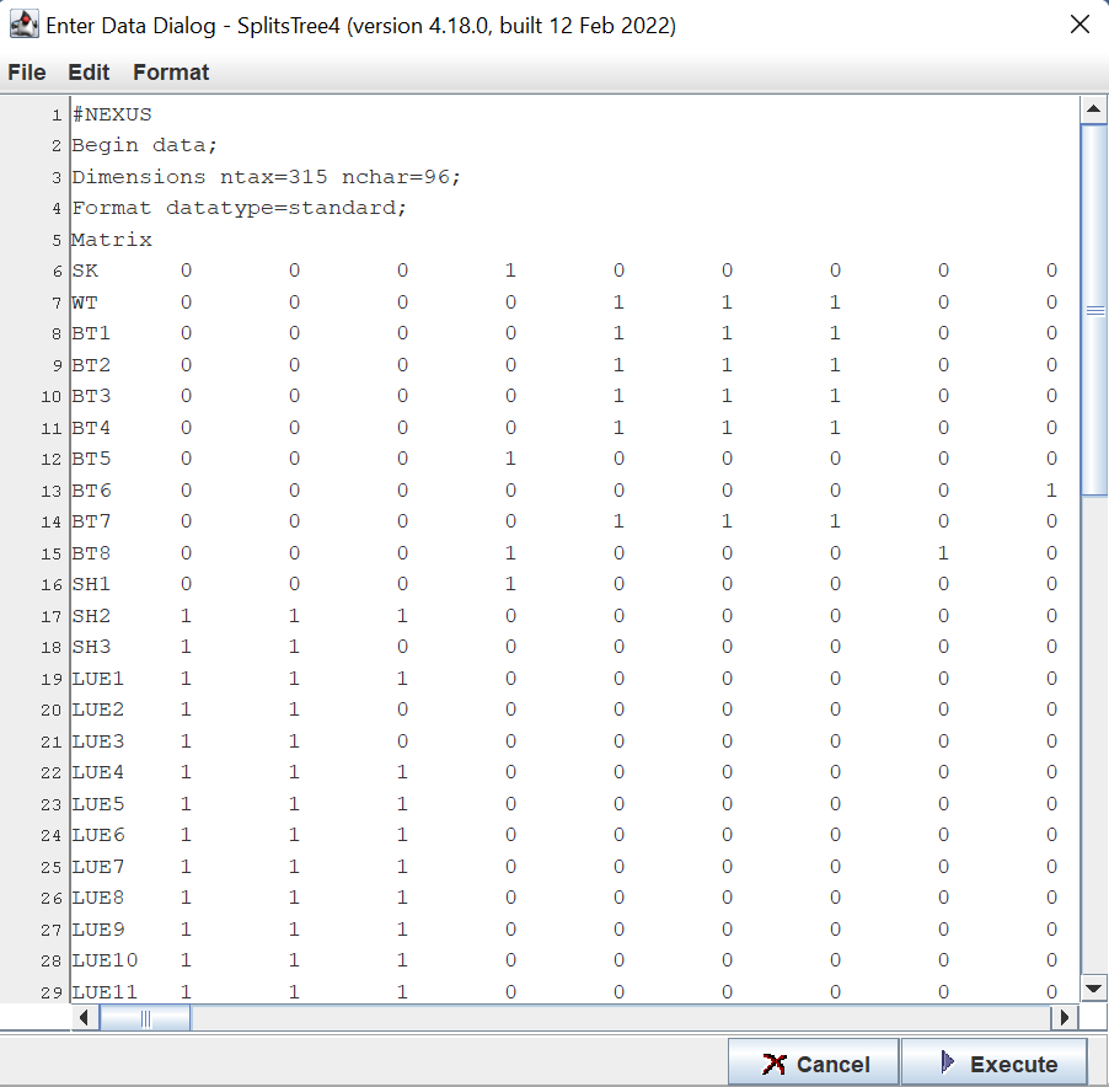
\includegraphics[width=\textwidth]{yurayong-img005.png}
\caption{\label{fig:yurayong:5}The nexus-formatted data for computational modelling.}
\end{figure}



\subsubsection{Step 4: From nexus format to Neighbor-Net diagram}
\label{sec:yurayong:3.2.4}
The final step of the data illustration process involves feeding the organised data, previously formatted according to the nexus format, into the software SplitsTree4 (version 4.18.0, built on 12 February 2022). This software operates using the Neighbor-Net algorithm, and by executing the imported data (as exemplified in \figref{fig:yurayong:5}), the software performs calculations and generates visual representations of the distances across tonological profiles of each dialect. The calculations also generate clustering of datapoints with similar profiles beneath the same nodes creating a clear illustration of the relationships, as illustrated in \figref{fig:yurayong:6}.

  
\begin{figure}
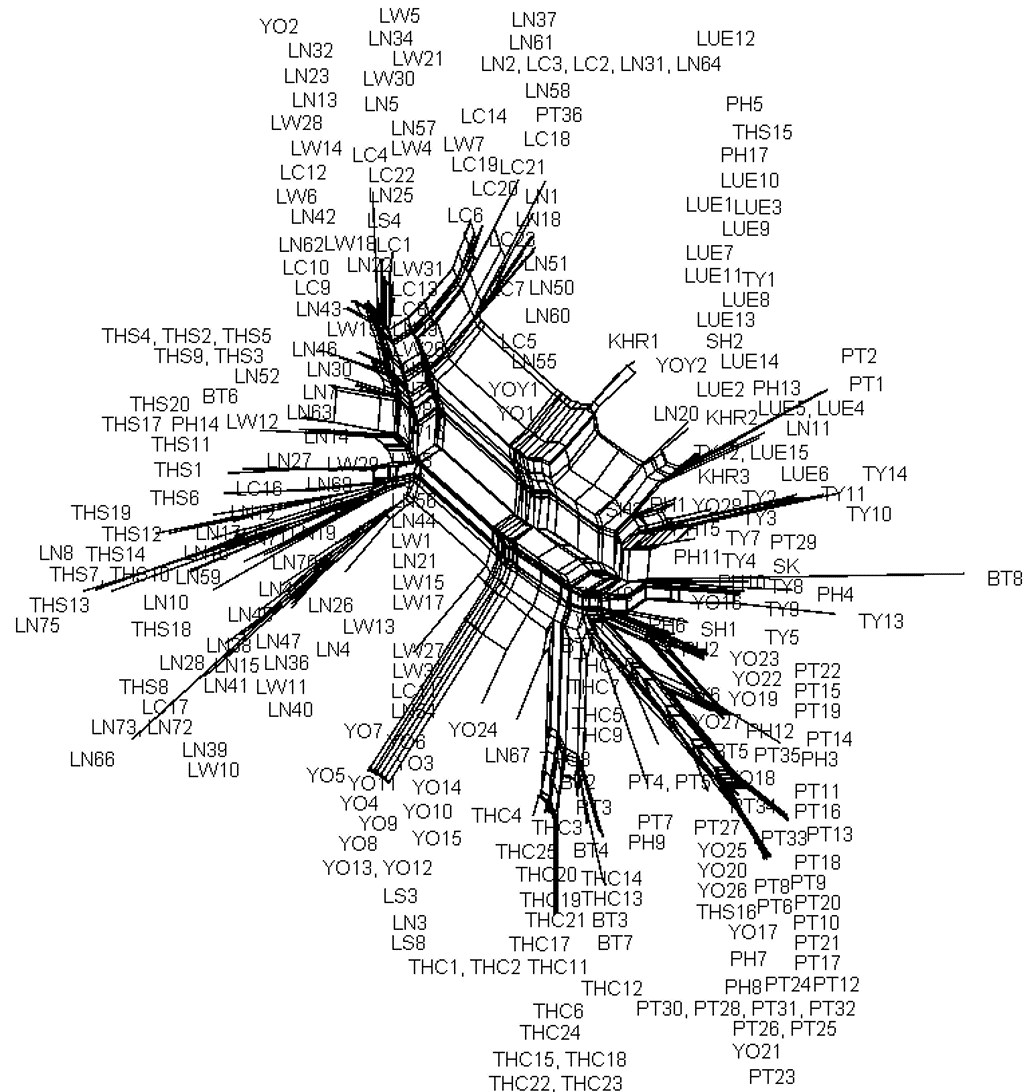
\includegraphics[width=\textwidth]{yurayong-img006.png}
\caption{\label{fig:yurayong:6}Neighbor-Net diagram for the tonological profiles of Tai dialects (n=315): LUE = Tai Lue; TY = Tai Yuan\slash Northern Thai; PT = Phu Thai; LN = Northern Lao; LC = Central Lao; LS = Southern Lao; LW = Western Lao\slash Northeastern Thai; THC = Central Thai; THS = Southern Thai; SK = Saek; SH = Shan; WT = White Tai; BT = Black Tai; YO = Yo; YOY = Yoy; PH = Phuan; KHR = Khorat Thai.}
\end{figure}

At this point, the computer-aided tools have fulfilled their role on the quantitative front, presenting the data in a visually interpretable fashion. The subsequent work phase involves a qualitative analysis based on the Tai-Kadai linguistics scholarship. This qualitative account seeks to identify significant signals which may be indicative of language changes.

\section{Data interpretation and discussion}
\label{sec:yurayong:4}
Through the Neighbor-Net diagram generated by the SplitsTree software (see \figref{fig:yurayong:6}), several distinct dialect clusters can be identified. These clusters are discernible by the presence of dominant dialects indicated in the list below, and as annotated with different colours and arranged in an anti-clockwise direction within \figref{fig:yurayong:7}.

\begin{multicols}{2}
\begin{enumerate}
\item Lao proper: LC, LS, LW
\item Southern Thai: THS    
\item Northern Lao: LN      
\item Yo: YO            
\item Central Thai: THC
\item Phu Thai: PT
\item Tai Yuan: TY
\item Tai Lue: LUE
\end{enumerate}
\end{multicols}
  
\begin{figure}
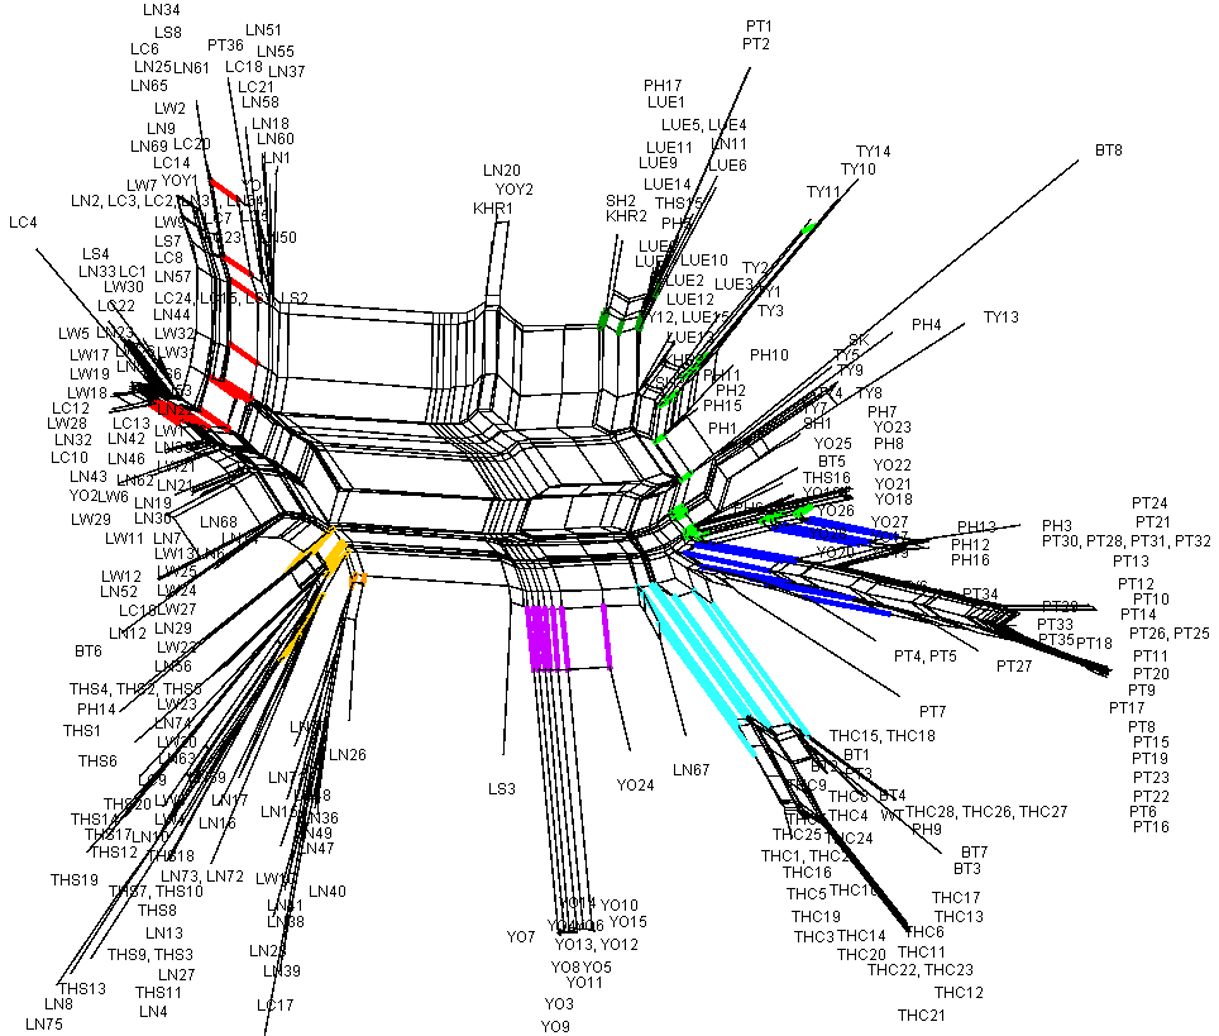
\includegraphics[width=\textwidth]{yurayong-img007.png}
\caption{\label{fig:yurayong:7} A Neighbor-Net diagram for the tonological profiles of Tai dialects (n=315) with identified clusters: LUE = Tai Lue; TY = Tai Yuan\slash Northern Thai; PT = Phu Thai; LN = Northern Lao; LC = Central Lao; LS = Southern Lao; LW = Western Lao\slash Northeastern Thai; THC = Central Thai; THS = Southern Thai; SK = Saek; SH = Shan; WT = White Tai; BT = Black Tai; YO = Yo; YOY = Yoy; PH = Phuan; KHR = Khorat Thai.}
\end{figure}

In general, the results largely agree with the genealogical classification proposed in the previous studies, as discussed in \sectref{sec:yurayong:1}. By identifying dialects which do not belong to their respective genealogical cluster based on the histori\hyp cal-comparative basis, we look further into their current speaking areas on the map and migration history of their respective speech communities. In this context, two specific cases will be discussed as illustrative examples.

First, the Central Lao dialect speaker LN11 is situated within a convergence of the Tai Yuan and Lue clusters, as noted in \figref{fig:yurayong:8}. As highlighted on the map using a red circle, the Northern Lao dialect LN11 is presently spoken within the major Tai Yuan and Lue speaking areas.

 
\begin{figure}
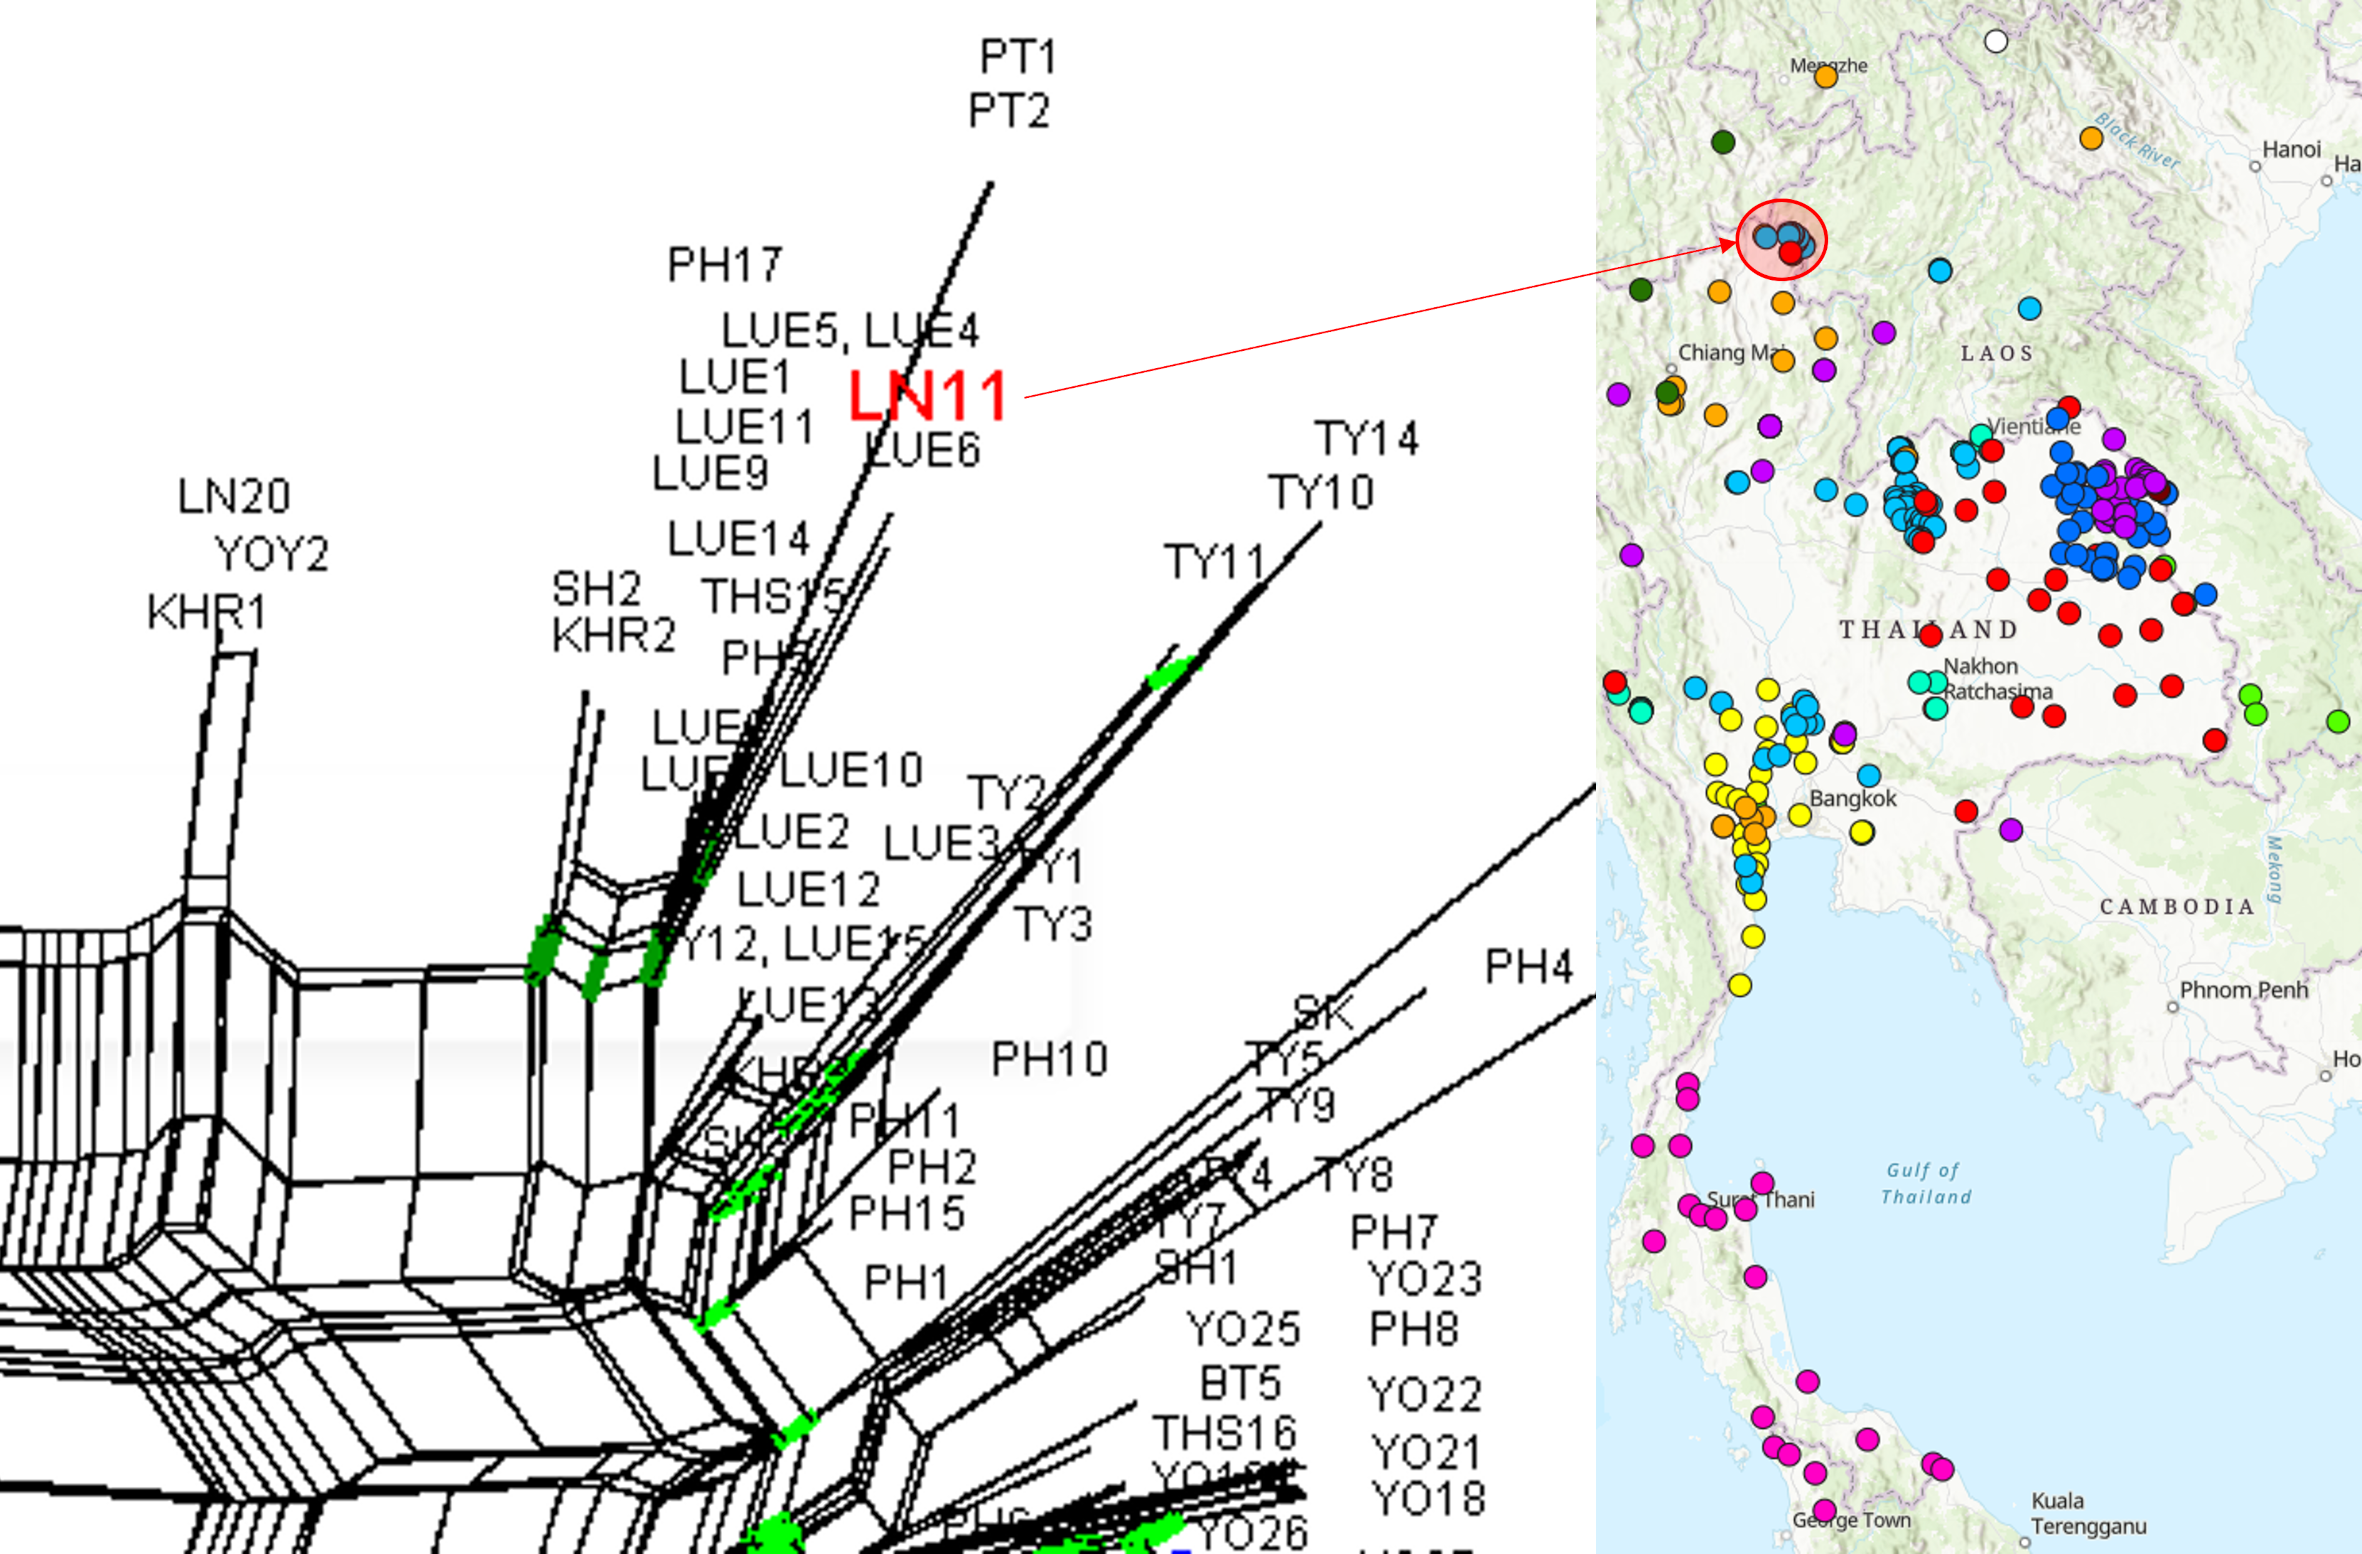
\includegraphics[width=\textwidth]{yurayong-img008.png}
\caption{\label{fig:yurayong:8}The Northern Lao dialect speaker (LN11) in Chiang Khong, Chiang Rai province, Thailand.}
\end{figure}

Second, the Central Lao dialect speaker LN67 aligns with the Central Thai cluster, as indicated by a red circle in \figref{fig:yurayong:9}. By examining the map, the location of the Northern Lao dialect LN67 is currently situated adjacent to the major speaking areas of Central Thai dialects.

 
\begin{figure}
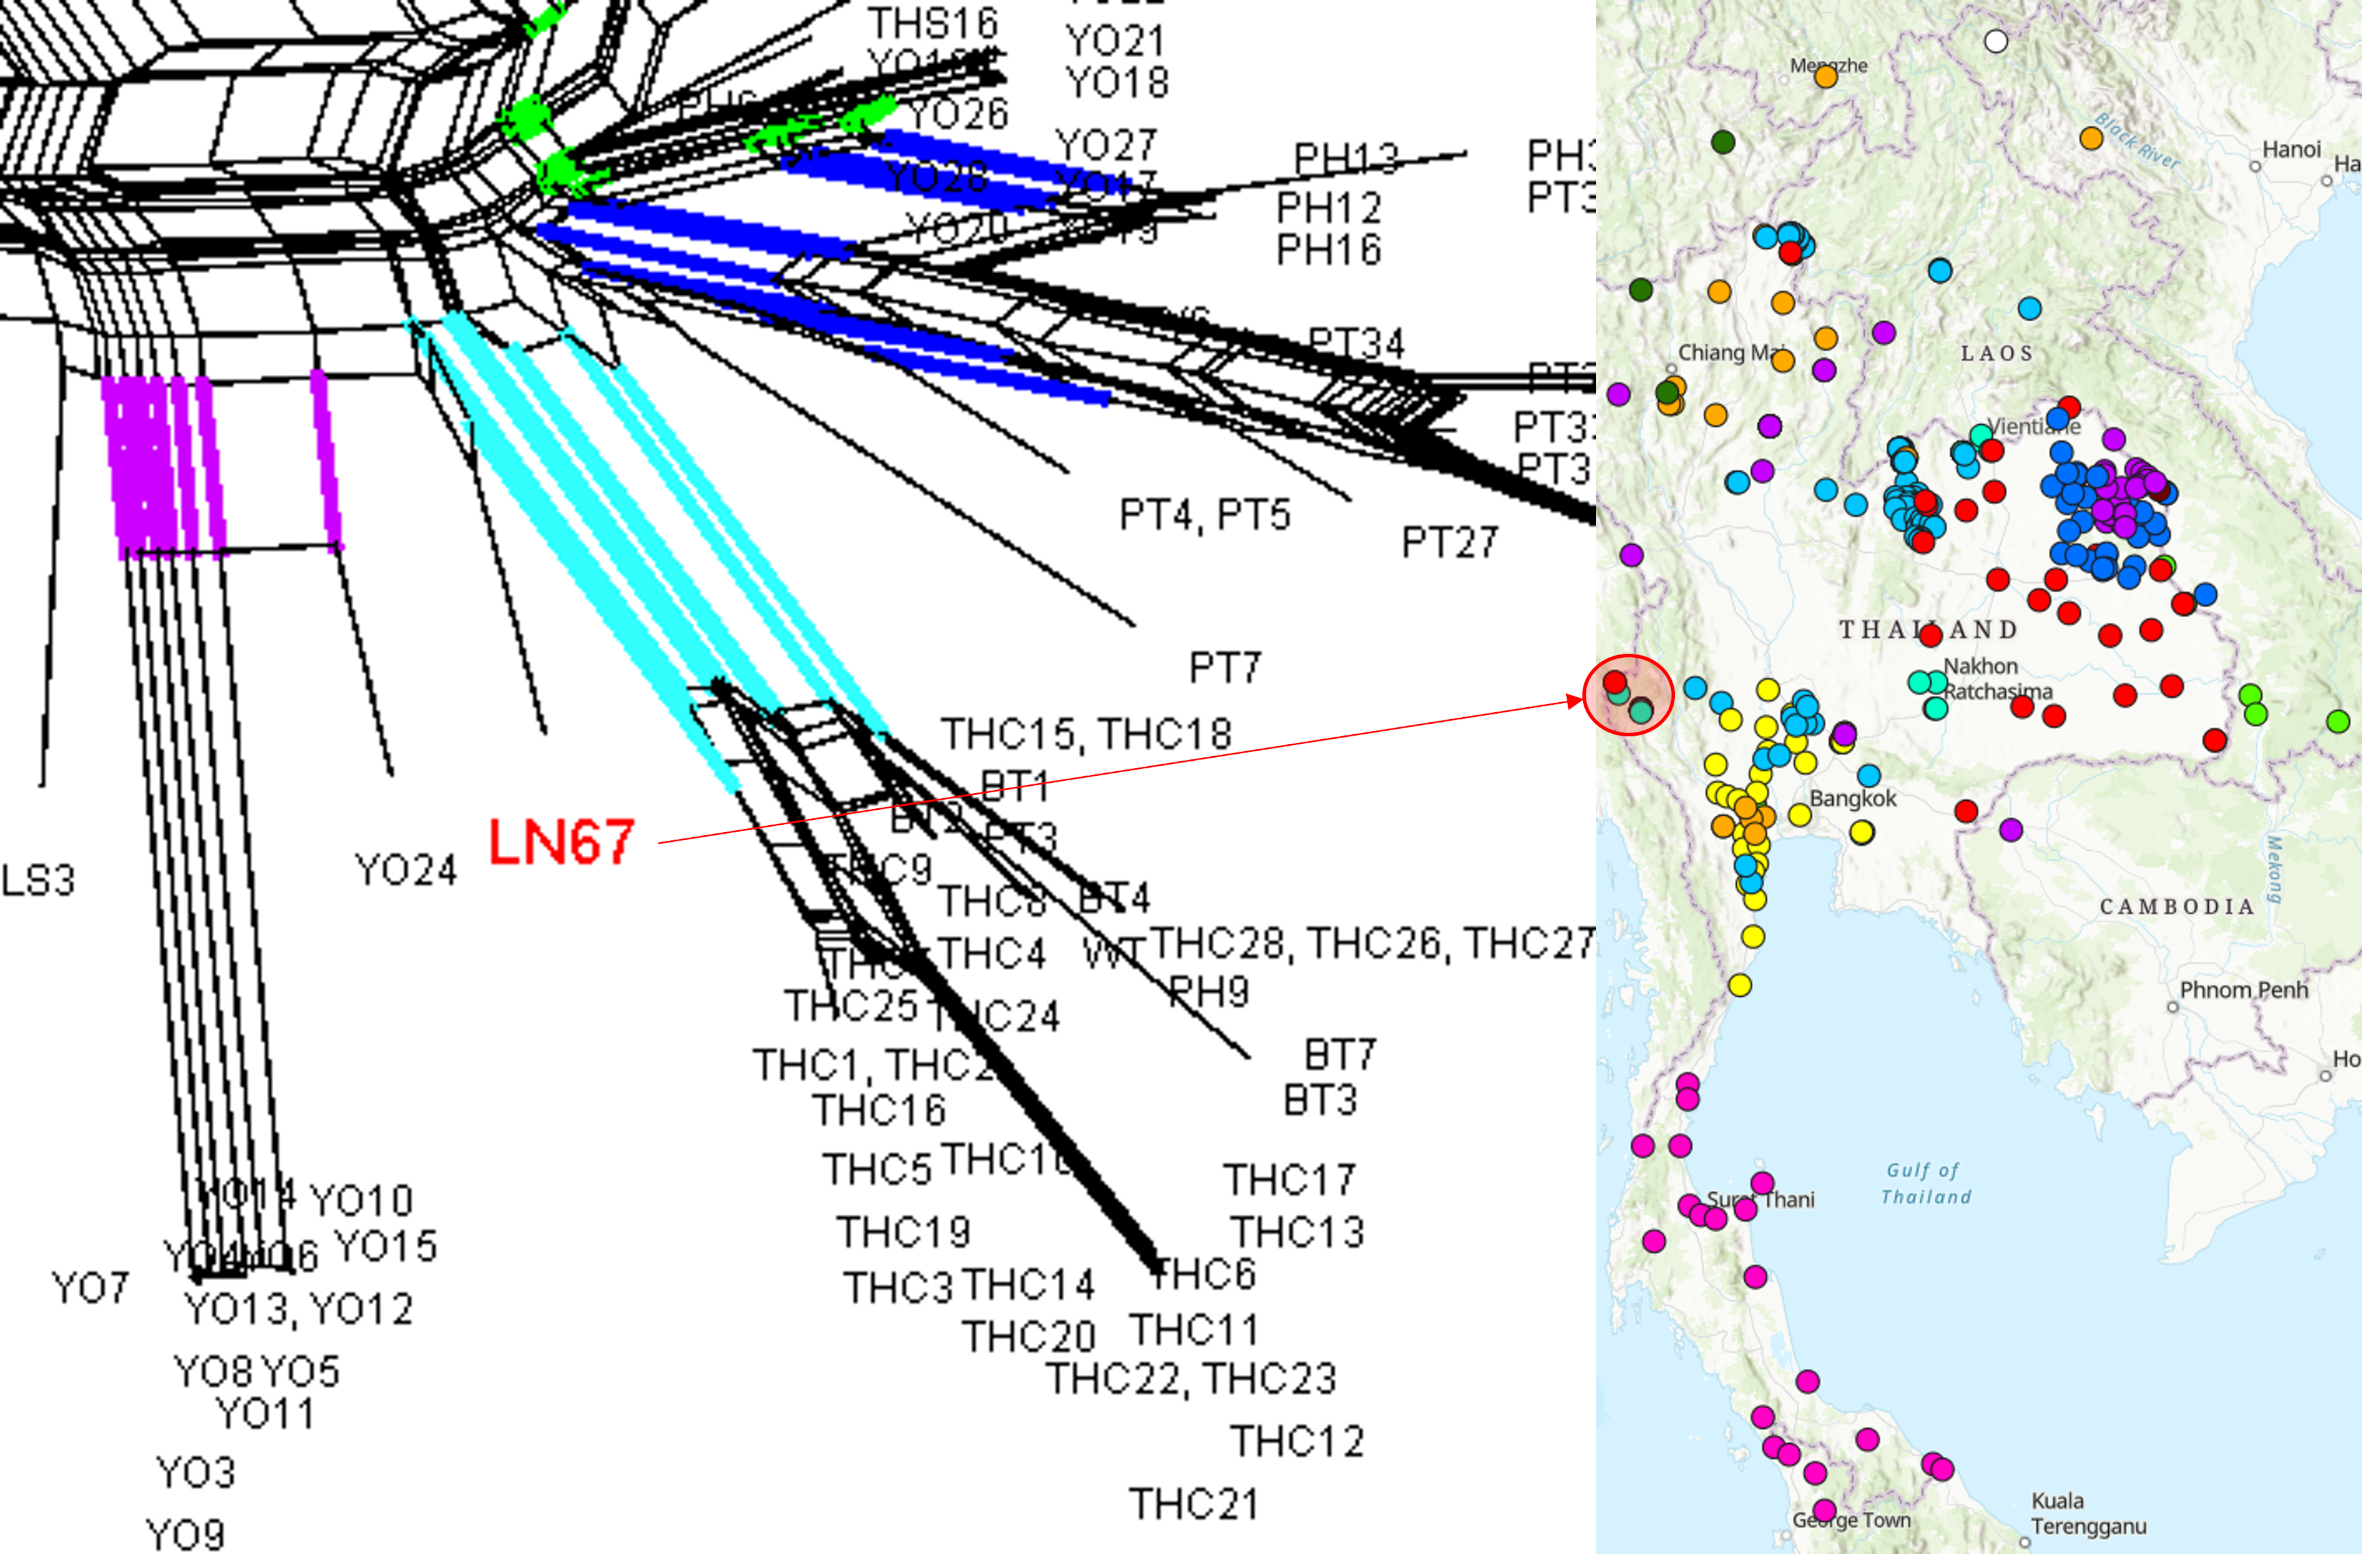
\includegraphics[width=\textwidth]{yurayong-img009.png}
\caption{\label{fig:yurayong:9}The Northern Lao dialect speaker (LN67) in Sangkhlaburi, Kanchanaburi province, Thailand.}
\end{figure}

Both of the aforementioned cases highlight a scenario where the examined dialects have undergone or are undergoing a shift in their homophonous tone pattern of DL and DS. This shift reflects a convergence towards the tonal profile of a regional dialect within their newly settled area, in line with their sociocultural assimilation. This phenomenon can be effectively demonstrated by comparing their tone paradigms with our reconstructed common Lao tone system in \tabref{tab:yurayong:8}, serving as a baseline.

\begin{table}
% \begin{tabular}{l *5{r} }
% \lsptoprule
% Initial consonant class at & \\
% time of tonal splits       & A & B & C & DL & DS\\\midrule
% Aspirated & 1 & 4 & 5 & 5 & 1\\
% Plain     & 2 &   &   &   & \\
% Implosive &   &   &   &   & \\
% Voiced    & 3 &   & 6 & 6 & 4\\
% \lspbottomrule
% \end{tabular}

\includegraphics[scale=.8]{20240810 grafiken yurayong neu/Table 8.png}
\caption{A reconstructed tone paradigm of common Lao.}
\label{tab:yurayong:8}
\end{table}

\clearpage
There are two major characteristics of Lao tone paradigms in general and across dialects which have been, respectively, retained and undergone changes in the two dialects under investigation. The first feature is found within tone B where there is no distinction between the original initial consonant classes (as discussed in \sectref{sec:yurayong:2}, \tabref{tab:yurayong:5}). The second hallmark of the Lao tone paradigm is what is labelled in Tai-Kadai linguistics as the Lao ladders, which concerns the paradigmatic distribution of tones within tones C and DL, as marked in bold in \tabref{tab:yurayong:8}.

On the one hand, the primary attribute of tone B remains largely intact across the majority of contemporary Lao dialects, including the two diaspora dialects under investigation (see Tables~\ref{tab:yurayong:9} and~\ref{tab:yurayong:10}), irrespective of the geographical locations of their current speaking areas. Accordingly, \citet[337]{Akkharawatthanakun2003} observes that the split of tone B4 from tones B123 in any Lao dialects can be considered a strong indication of deviation from the common Lao pattern, as is evident in the case of Khorat Thai dialects regarded as hybrid dialects of Western Lao and Central Thai.

On the other hand, the second homophonous pattern between tones C and DL is gradually fading away within the two Northern Lao dialects under investigation. These dialects are spoken outside their core regions around Luang Phrabang in Northern Laos, as can be observed from the tone paradigms given in Tables~\ref{tab:yurayong:9} and \ref{tab:yurayong:10}.


\begin{table}
% \begin{tabular}{l *5{r} }
% \lsptoprule
% Initial consonant class at & \\
% time of tonal splits       & A & B & C & DL & DS\\\midrule
% Aspirated & 1 & 3 & 4 & 3 & 1\\
% Plain     &   &   & 5 &   & \\
% Implosive &   &   &   &   & \\
% Voiced    & 2 &   & 4 & 6 & 3\\
% \lspbottomrule
% \end{tabular}

\includegraphics[scale=.8]{20240810 grafiken yurayong neu/Table 9.png}
\caption{Tone paradigm of the Northern Lao dialect speaker (LN11) in Chiang Khong, Chiang Rai province, Thailand.}
\label{tab:yurayong:9}
\end{table}


\begin{table}
% \begin{tabular}{l *5{r} }
% \lsptoprule
% Initial consonant class at & \\
% time of tonal splits & A & B & C & DL & DS\\\midrule
% Aspirated & 1 & 3 & 4 & 3 & 6\\
% Plain & 2 &  &  &  & \\
% Implosive &  &  &  &  & 5\\
% Voiced &  &  & 5 & 4 & 7\\
% \lspbottomrule
% \end{tabular}

\includegraphics[scale=.8]{20240810 grafiken yurayong neu/Table 10.png}
\caption{Tone paradigm of the Northern Lao dialect speaker (LN67) in Sangkhlaburi, Kanchanaburi province, Thailand.}
\label{tab:yurayong:10}
\end{table}

Our hypothesis is that the occurrence of a paradigmatic shift is ongoing, indicating a trend converging towards the tonal profiles prevalent in other Tai dialects, which are predominantly spoken by the majority populations in the areas. In order to assess the validity of our hypothesis, a comparative analysis is conducted using two additional baselines: Tai Yuan (\tabref{tab:yurayong:11}) and Central Thai (\tabref{tab:yurayong:12}).


\begin{table}
% \begin{tabular}{ l *5{r} }
% \lsptoprule
% Initial consonant class at & \\
% time of tonal splits & A & B & C & DL & DS\\\midrule
% Aspirated & 1 & 3 & 5 & 3 & 1\\
% Plain &  &  &  &  & \\
% Implosive & 2 &  &  &  & \\
% Voiced &  & 4 & 6 & 4 & 5\\
% \lspbottomrule
% \end{tabular}

\includegraphics[scale=.8]{20240810 grafiken yurayong neu/Table 11.png}
\caption{Tone paradigm of common Tai Yuan.}
\label{tab:yurayong:11}
\end{table}

\begin{table}
% \begin{tabular}{ l *5{c} }
% \lsptoprule
% Initial consonant class at & \\
% time of tonal splits & A & B & C & DL & DS\\\midrule
% Aspirated & 5 & 2 & 3 & 2 & 2\\
% Plain & 1 &  &  &  & \\
% Implosive &  &  &  &  & \\
% Voiced & (6) & 3 & 4 & 3 & 4\\
% \lspbottomrule
% \end{tabular}

\includegraphics[scale=.8]{20240810 grafiken yurayong neu/Table 12.png}
\caption{Tone paradigm of common Central Thai.}
\label{tab:yurayong:12}
\end{table}

Upon comparing the paradigms of common Tai Yuan and common Central Thai with those present in the two Northern Lao dialects, it is obvious that the Lao ladders have been decomposed within the two diaspora dialects under investigation. Another observation pertains to tone A, wherein the Northern Lao dialect speaker in Sangkhlaburi (LN67) seems to have adopted a splitting pattern akin to that of Central Thai. This adaptation results in a differentiation of tone A1 (originating from aspirated initials) from the other tones, A234, within the paradigm.

Furthermore, we assess the significance of language contact by considering the sociolinguistic context of the two Northern Lao dialect speakers within the diaspora: LN11 and LN67. Although \citet{Akkharawatthanakun2003} does not explicitly report the extent of contact intensity and the specific domains of usage for both dialects, it is highly likely that bilingualism has resulted in the reorganisation and convergence of homophonous patterns within the Northern Lao tone paradigm towards the dominant regional dialects in their respective locations. In the case of LN11, this particular Northern Lao dialect speaker has primarily resided in the border region between northwestern Laos and northern Thailand on the Thai side, where the dominant regional language is Tai Yuan \citep[150, 450]{Akkharawatthanakun2003}. Similarly, the living environment of the Northern Lao dialect speaker LN67 involves contact with Central Thai, the dominant regional language in western Thailand, as well as with other diasporic Lao dialects \citep[150, 448]{Akkharawatthanakun2003}.

Based on our tonological profile data (as shown in Tables~\ref{tab:yurayong:9} and~\ref{tab:yurayong:10}), exposure to Tai Yuan and Central Thai speaking environments, respectively, emerges as a highly plausible factor contributing to the decomposition of the Lao ladders within tones C and DL. Additionally, the Central Thai tone paradigm also provides a model for the reorganisation of tone slots within tone A for the Northern Lao dialect speaker LN67 (as discussed above). At the same time, it appears that homogeneity within the common Lao tones B1234 (as highlighted in Tables~\ref{tab:yurayong:5} and~\ref{tab:yurayong:8}) remains stable and resistant to contact-induced changes in the tone paradigm of these two speakers.

As a supplementary remark, we may also consider a language-internal perspective and posit a hypothesis that tones DL and DS paradigmatically and cognitively lie at a deeper level of prominence and speaker’s awareness. This heightened prominence might stem from their vague status within the tone paradigm and the variations observed among individual dialect speakers, due to their probabilistic status as a low-frequency syllable type and a low-probable tone type in the language system (see e.g. the case of Chinese dialects in \citealt{WienerIto2015}). Consequently, these distinctive characteristics may make them more prone to alternation and change when compared to the salient tones A, B, and C, which are often emphasised in the process of acquisition, more systematically taught in school and acquired by children from their elementary education. This scenario is usually observed in the teaching of standard languages, Lao and Thai, as well as Vietnamese, Cantonese and Mandarin (see e.g. \citealt{Bar-Lev1991}). However, the method used in the current study is not specifically designed to test this particular claim. Nevertheless, this aspect can offer an interesting direction for future research which could bridge the domains of dialectology and cognitive sciences. Such exploration could provide valuable insights into the dynamics of tone paradigms and their evolution.

\section{Conclusions}
\label{sec:yurayong:5}
In the present study, we have examined and discussed instances of language shift occurring in various regions where Tai dialect speakers are shifting their language whose tone paradigm structure subsequently also converges with a dominant regional dialect. From the perspective of tone paradigm, the convergence has sometimes resulted in the emergence of transitional dialect systems, in which a protosystem has undergone restructuring, aligning itself more closely with the model provided by the dominant regional dialect. These transitional dialect systems of tone paradigm stand out when examined through a quantitative approach in combination with the conventional comparative method. It enables identification of the protostructure of tone paradigm from which the transitional dialect systems have diverged. In any case, our results do not post significant challenges to the genealogical classification proposed in the previous studies, as the signals of change observed in the present study primarily pertain to contact-induced changes occurring subsequent to the dispersal stages of individual Tai subbranches.

At a methodological level, we have also demonstrated the utility of Neighbor-Net algorithm as an effective tool for identifying such instances from a big pool of data. Our method employed to gather, organise and analyse the data can potentially offer a preliminary model for scholars engaged in the studies of Tai dialects as well as for those researching dialects of other Mainland Southeast Asian languages with tones. As more data, particularly relating to tone paradigms, have been continuously collected from field during the recent decades, this methodological model should also facilitate scholars and dialectological studies with a focus on tonal aspects in embracing an emerging trend within digital humanities and big data studies.

Lastly, our vital message to scholars engaged in language documentation and description is that the collection of sociolinguistic data stands on equal footing with the description of language features. From the present study, we see that insufficient description of sociolinguistic context regarding informants may pose a challenge when attempting to establish a contact-based explanation for a language change. With the inclusion of such comprehensive sociolinguistic information about the speakers, their speech communities and their linguistic repertoires, numerous finely-tuned analyses centred around cross-factor correlations can yield significantly more insightful understanding of the language situation. Such analyses will contribute to the discussion of language change and the diversification of dialects, a dynamic process which continues to evolve as we advance into the 21st century.

\section*{Abbreviations}

\subsection*{Tones}
\begin{tabbing}
MM \= Tone A\kill
A  \> Tone A, smooth syllable\\ 
B  \> Tone B, smooth syllable\\ 
C  \> Tone C, smooth syllable\\
DL \> Tone D, long vowel, checked syllable\\ 
DS \> Tone D, short vowel, checked syllable
\end{tabbing}

\subsection*{Languages}
\begin{multicols}{2}
\begin{tabbing}
MMM \= Black Tai\kill
BT \> Black Tai\\
KHR \> Khorat Thai\\
LC \> Central Lao\\
LN \> Northern Lao\\
LS \> Southern Lao\\
LUE \> Tai Lue\\
LW \> Western Lao\slash Northeastern Thai\\
PH \> Phuan\\
PT \> Phu Thai\\
SH \> Shan\\
SK \> Saek\\
THC \> Central Thai\\
THS \> Southern Thai\\
TY \> Tai Yuan\slash Northern Thai\\
WT \> White Tai\\
YO \> Yo\\
YOY \> Yoy
\end{tabbing}
\end{multicols}

\section*{Acknowledgements}

This research was supported by the Grant for Graduate Student 2021 from the King Prajadhipok and Queen Rambhai Barni Memorial Foundation, awarded to Saknarin Pimvunkum for the research project
“Classification of Vientiane Lao dialects in Western Thailand by tone paradigm” and was part of the project “Northeast and Southeast Asian Studies Network in Finland and Thailand (NSEANET)” funded by the Finnish National Agency for Education (EDUFI) during 2020–2023. This study was exempted from ethical review by the Committee for Research Ethics (Social Sciences), Faculty of Social Sciences and Humanities, Mahidol University (2022/001.1701, 17 January 2022).

\printbibliography[heading=subbibliography,notkeyword=this]
\end{document}

% @phdthesis{Akkharawatthanakun2003,
% 	author = {Akkharawatthanakun, Phinnarat},
% 	school = {A case study of the Lao language} (Doctoral},
% 	year = {2003}
% }s
% 
% 
% @article{Akkharawatthanakun2020,
% 	author = {Akkharawatthanakun, Phinnarat},
% 	journal = {\textit{Journal of Liberal Arts}},
% 	note = {. \url{https://doi.org/10.14456/lartstu.2020.31}},      
% 	number = {2},
% 	pages = {513–548},
% 	title = {Tonal Diversity and Tone Sandhi in Lue},
% 	volume = {20},
% 	year = {2020}
% }
% 
% 
% @article{Bar-Lev1991,
% 	author = {Bar-Lev, Zev},
% 	journal = {\textit{Journal of the Chinese Language Teachers Association}},
% 	note = {. \url{https://eric.ed.gov/?id=EJ447341}},
% 	number = {3},
% 	pages = {1–24},
% 	title = {Two Innovations for Teaching Tones},
% 	volume = {26},
% 	year = {1991}
% }
% 
% 
% @book{Brown1985,
% 	address = {Bangkok},
% 	author = {Brown, J. Marvin},
% 	publisher = {White Lotus},
% 	title = {\textit{From Ancient {Thai} to Modern Dialects}},
% 	year = {1985}
% }
% 
% 
% @article{BryantBryant2004,
% 	author = {Bryant, David and Vincent Moulton},
% 	journal = {\textit{Molecular Biology and Evolution}},
% 	note = {. \url{https://doi.org/10.1093/molbev/msh018}},  
% 	number = {2},
% 	pages = {255–265},
% 	title = {Neighbor-Net: {{A}}n agglomerative method for the construction of phylogenetic networks},
% 	volume = {21},
% 	year = {2004}
% }
% 
% 
% @article{BunyasathitBunyasathit2016,
% 	author = {Bunyasathit, Wannaporn, Chantas Pientam and Theptida Silapabanleng},
% 	journal = {\textit{Journal of Nakhonratchasima College}},
% 	note = {. \url{http://journal.nmc.ac.th/th/admin/Journal/2560Vol11No1_702.pdf}},
% 	number = {1},
% 	pages = {26–38},
% 	title = {The Historical Development of {LaoW}iang People in {{{U}}} Thong District, {Suphanburi} Province},
% 	volume = {11},
% 	year = {2016}
% }
% 
% 
% @article{Burusphat2012,
% 	author = {Burusphat, Somsonge},
% 	journal = {\textit{Journal of the Southeast Asian Linguistics Society}},
% 	note = {. \url{http://hdl.handle.net/1885/9118}},
% 	pages = {32–48},
% 	title = {Tones of {Thai Song} varieties},
% 	volume = {5},
% 	year = {2012}
% }
% 
% 
% @book{Canilao2010,
% 	address = {Nakhon Pathom},
% 	author = {Canilao, Kritsana},
% 	note = {\url{http://mulinet11.li.mahidol.ac.th/e-thesis/2553/cd446.1/4836363.pdf}},
% 	publisher = {Mahidol University},
% 	title = {\textit{Tonal Geography of the Provinces of {Central} {Thailand}} (Doctoral dissertation)},
% 	year = {2010}
% }
% 
% 
% Chamberlain, James R. 1975. A new look at the history and classification of the Tai languages. In Jimmy G. Harris \& James R. Chamberlain (eds.), \textit{Studies in Tai linguistics in honor of William J. Gedney}, 49–66. Central Institute of English Language. \url{http://sealang.net/sala/archives/pdf8/chamberlain1975new.pdf}
% 
% @incollection{Damanhuri2004,
% 	address = {Tempe, AZ},
% 	author = {Damanhuri, Umaiyah},
% 	booktitle = {\textit{Papers from the Eleventh Annual Meeting of the {Southeast} {Asian} Linguistics Society, Tempe, {Arizona}}},
% 	editor = {Somsonge Burusphat},
% 	note = { \url{http://sealang.net/sala/archives/pdf4/damanhuri2004classification.pdf}},
% 	pages = {167–182},
% 	publisher = {Arizona State University},
% 	title = {The classification of some {Thai} dialects spoken in {Kedah}},
% 	year = {2004}
% }
% 
% 
% @phdthesis{Dockum2019,
% 	author = {Dockum, Rikker},
% 	school = {Tai tone in historical perspective} (Doctoral},
% 	year = {2019}
% }
% 
% 
% @incollection{Edmondson1990,
% 	address = {Arlington, TX},
% 	author = {Edmondson, Jerold A.},
% 	booktitle = {\textit{Development and diversity: {{L}}anguage variation across time and space (A {Festschrift} for {Charles}-{James} N. {{B}}ailey)}},
% 	editor = {Jerold A. Edmondson, Crawford Feagin and Peter Mühlhäusler},
% 	note = {\url{},
% 	pages = {187–202},
% 	publisher = {Summer Institute of Linguistics},
% 	title = {Kam tone splits and the variation of breathiness},
% 	url = {https://www.sil.org/resources/archives/8425}},
% 	year = {1990}
% }
% 
% 

% 
% 
% @incollection{Ferlus2004,
% 	address = {Tempe, AZ},
% 	author = {Ferlus, Michel},
% 	booktitle = {\textit{Papers from the Eleventh Annual Meeting of the {Southeast} {Asian} Linguistics \citealt{Society2001}}},
% 	editor = {Somsonge Burusphat},
% 	note = { \url{http://sealang.net/sala/archives/pdf8/ferlus2004origin.pdf}},
% 	pages = {297–313},
% 	publisher = {Arizona State University Programme for Southeast Asian Studies Monograph Series Press},
% 	title = {The origin of tones in Viet-Muong},
% 	year = {2004}
% }
% 
% 
% @incollection{Gedney1972,
% 	address = {The Hague},
% 	author = {Gedney, William J.},
% 	booktitle = {\textit{Studies in linguistics in honor of George L. {{T}}rager}},
% 	editor = {M. Estellie Smith},
% 	pages = {423–437},
% 	publisher = {Mouton de Gruyter},
% 	title = {A checklist for determining tones in {Tai} dialects},
% 	year = {1972}
% }
% 
% 
% @article{GrünthalGrünthal2016,
% 	author = {Grünthal, Riho and Johanna Nichols},
% 	journal = {\textit{Lingua Posnaniensis}},
% 	note = {. \url{https://doi.org/10.1515/linpo-2016-0008}},   
% 	number = {2},
% 	pages = {11–31},
% 	sortname = {Grunthal, Riho and Johanna Nichols},
% 	title = {Transitivizing-detransitivizing typology and language family history},
% 	volume = {58},
% 	year = {2016}
% }
% 
% 
% Handel, Zev. 2014. Historical Phonology of Chinese. In C. J. Huang, Y. A. Li, \& A. Simpson (eds.),~\textit{The Handbook of Chinese Linguistics}, 576–598. Oxford: John Wiley \& Sons.
% 
% @incollection{Hartmann2008,
% 	address = {London},
% 	author = {Hartmann, John F.},
% 	booktitle = {\textit{The {Tai}-Kadai Languages}},
% 	editor = {Anthony V. N. Diller, Jerold A. Edmondson and Yongxian Luo},
% 	pages = {254–297},
% 	publisher = {Routledge},
% 	title = {The Lue Language},
% 	year = {2008}
% }
% 
% 
% @article{Haudricourt1954,
% 	author = {Haudricourt, André-Georges},
% 	journal = {\textit{Journal Asiatique}},
% 	note = {. \url{https://lacito.hypotheses.org/files/2015/12/Haudricourt_1954_Origine-Tons-Vietnamien_scan.pdf}},
% 	pages = {69–82},
% 	sortname = {Haudricourt, Andre-Georges},
% 	title = {De l’origine des tons en vietnamien},
% 	volume = {242},
% 	year = {1954}
% }
% 
% 
% @book{Hill2019,
% 	address = {Cambridge},
% 	author = {Hill, Nathan},
% 	publisher = {Cambridge University Press},
% 	title = {\textit{The Historical Phonology of {Tibetan}, {Burmese}, and {Chinese}}},
% 	year = {2019}
% }
% 
% 
% @book{Hudak2008,
% 	address = {Gedney’s Comparative Tai Source Book}. Honolulu, HI},
% 	author = {Hudak, Thomas John},
% 	note = {\url{},
% 	publisher = {University of Hawai’i Press},
% 	title = {\textit{William J},
% 	url = {https://www.jstor.org/stable/20532978}},
% 	year = {2008}
% }
% 
% 
% @article{HusonHuson2006,
% 	author = {Huson, Daniel H. and David Bryant},
% 	journal = {\textit{Molecular Biology and Evolution}},
% 	note = {. \url{https://doi.org/10.1093/molbev/msj030}},   
% 	number = {2},
% 	pages = {254–267},
% 	title = {Application of phylogenetic networks in evolutionary studies},
% 	volume = {23},
% 	year = {2006}
% }
% 
% 
% @incollection{Kingston2011,
% 	address = {Oxford},
% 	author = {Kingston, John},
% 	booktitle = {\textit{The {Blackwell} companion to phonology}},
% 	editor = {Marc van Oostendorp, Colin J. Ewen, Elizabeth Hume and Keren Rice},
% 	note = { \url{https://doi.org/10.1002/9781444335262.wbctp0097}},  
% 	pages = {2304–2333},
% 	publisher = {Wiley-Blackwell},
% 	title = {Tonogenesis},
% 	year = {2011}
% }
% 
% 
% @book{Koowatthanasiri1981,
% 	address = {Bangkok},
% 	author = {Koowatthanasiri, Kanjana},
% 	note = {\url{http://cuir.car.chula.ac.th/handle/123456789/35801}},
% 	publisher = {Chulalongkorn University},
% 	title = {\textit{The Tones of Nyo} (Master’s thesis)},
% 	year = {1981}
% }
% 
% 
% @book{Li1977,
% 	address = {Manoa, HI},
% 	author = {Li, Fang-Kuei},
% 	note = {\url{},
% 	publisher = {University Press of Hawai’i},
% 	title = {\textit{A Handbook of Comparative {Tai}}},
% 	url = {https://www.jstor.org/stable/20006684}},
% 	year = {1977}
% }
% 
% 
% @book{LiangLiang1996,
% 	address = {Beijing},
% 	author = {Liang, Min and Junru Zhang},
% 	publisher = {China Social Sciences Publishing House},
% 	title = {\textit{Dòngtáiyǔ Gàilùn} [An introduction to the Kam-{Tai} Languages]},
% 	year = {1996}
% }
% 
% 
% @book{Liao2016,
% 	address = {Chiang Mai},
% 	author = {Liao, Hanbo},
% 	note = {\url{},
% 	publisher = {Payap University},
% 	title = {\textit{Tonal Development of {Tai} languages} (Master’s thesis)},
% 	url = {https://www.academia.edu/download/49907598/Final-TONAL_DEVELOPMENT_OF_TAI_LANGUAGES-0714.pdf}},
% 	year = {2016}
% }
% 
% 
% @book{Liao2023a,
% 	address = {\textit{Folia Linguistica}. Published online 2022-11-30},
% 	author = {Liao, Hanbo},
% 	note = {org/10.1515/flin-}},     
% 	publisher = {\url{https://doi},
% 	title = {An integrated tone box scheme for determining tones in {{Tai}} varieties beyond {Southwestern} {{Tai}}: {{D}}iachronic and synchronic concerns},
% 	urldate = {2022-2048},
% 	year = {2022}
% }
% 
% 
% @phdthesis{Liao2023b,
% 	author = {Liao, Hanbo},
% 	school = {typological structures and diachronic issues} (Doctoral},
% 	year = {2023}
% }
% 
% 
% @article{Luo1988,
% 	author = {Luo, Meizhen},
% 	journal = {\textit{Mínzú Yǔwén} [Minority Languages of China]},
% 	number = {2},
% 	pages = {26–34},
% 	title = {Dǎi Tài cíhuì bǐjiào [A comparison of Dai and {Thai} vocabularies]},
% 	volume = {1988},
% 	year = {1988}
% }
% 
% 
% @book{Luo1997,
% 	address = {Hong Kong},
% 	author = {Luo, Yongxian},
% 	note = {\url{},
% 	publisher = {The Chinese University of Hong Kong Press},
% 	title = {\textit{The subgroup structure of the {Tai} languages: {{A}} historical-comparative study}},
% 	url = {https://www.jstor.org/stable/23887080}},
% 	year = {1997}
% }
% 
% 
% @article{Maddieson1984,
% 	author = {Maddieson, Ian},
% 	journal = {\textit{Journal of Phonetics}},
% 	note = {. \url{https://doi.org/10.1016/S0095-4470(19)30845-9}},   
% 	number = {1},
% 	pages = {9--15},
% 	title = {The effects on F0 of a voicing distinction in sonorants and their implications for a theory of tonogenesis},
% 	volume = {12},
% 	year = {1984}
% }
% 
% 
% @article{MaddisonMaddison1997,
% 	author = {Maddison, David R., David L. Swofford and Wayne P. Maddison},
% 	journal = {\textit{Systematic Biology}},
% 	note = {. \url{https://doi.org/10.1093/sysbio/46.4.590}}, 
% 	number = {4},
% 	pages = {590–621},
% 	title = {Nexus: {{A}}n extensible file format for systematic information},
% 	volume = {46},
% 	year = {1997}
% }
% 
% 
% Michaud, Alexis \& Bonny Sands. 2020. Tonogenesis. In Mark Aronoff (ed.), \textit{Oxford Research Encyclopedia of Linguistics}. Oxford: Oxford University Press. \url{https://oxfordre.com/linguistics/view/10.1093/acrefore/9780199384655.001.0001/acrefore-9780199384655-e-748} 
% 
% @article{Mitani1977,
% 	author = {Mitani, Yasuyuki},
% 	journal = {\textit{Tōnan'ajia kenkyū} [Southeast Asian Studies]},
% 	note = {. \url{https://kyoto-seas.org/pdf/09.pdf}},
% 	number = {3},
% 	pages = {421–429},
% 	title = {{{Tai}}-Kadai shogo no gengonendaigaku-teki kōsatsu [Linguistic chronology of {{Tai}}-Kadai Languages]},
% 	urldate = {15/3/1503},
% 	volume = {15},
% 	year = {1977}
% }
% 
% 
% @incollection{Nichols2020,
% 	address = {Oxford},
% 	author = {Nichols, Johanna},
% 	booktitle = {\textit{Language dispersal, diversification, and contact: {{A}} global perspective}},
% 	editor = { Mily Crevels and Pieter Muysken},
% 	note = { \url{https://doi.org/10.1093/oso/23813.003.0002}},
% 	pages = {25–43},
% 	publisher = {Oxford University Press},
% 	title = {Dispersal patterns shape areal typology},
% 	urldate = {97801987},
% 	year = {2020}
% }
% 
% 
% @incollection{Ostapirat2005,
% 	address = {London},
% 	author = {Ostapirat, Weera},
% 	booktitle = {\textit{The peopling of {East} {Asia}: {{P}}utting together archaeology, linguistics and genetics}},
% 	editor = {Roger Blench, Laurent Sagart and Alicia Sanchez-Mazas},
% 	note = { \url{https://doi.org/10.4324/43685}},
% 	pages = {107–131},
% 	publisher = {Routledge},
% 	title = {Kra-dai and {Austronesian}: {{N}}otes on phonological correspondences and vocabulary distribution},
% 	urldate = {97802033},
% 	year = {2005}
% }
% 
% 
% @book{Pittayaporn2009,
% 	address = {Ithaca, NY},
% 	author = {Pittayaporn, Pittayawat},
% 	note = {\url{https://ecommons.cornell.edu/bitstream/handle/5/Pittayaporn,%20Pittayawat.pdf}},
% 	publisher = {Cornell University},
% 	title = {\textit{The phonology of Proto-{Tai}} (Doctoral dissertation)},
% 	urldate = {1813/1385},
% 	year = {2009}
% }
% 
% 
% @article{Pittayaporn2014,
% 	author = {Pittayaporn, Pittayawat},
% 	journal = {\textit{Manusya – Journal of Humanities}, Special issue},
% 	note = {. \url{https://doi.org/10.9077-01703004}},
% 	pages = {47–68},
% 	title = {Layer of {Chinese} loanwords in Proto-{{Southwestern}} {{Tai}} as evidence for the dating of the spread of {{Southwestern}} {{Tai}}},
% 	urldate = {1163/2665},
% 	volume = {20},
% 	year = {2014}
% }
% 
% 
% @book{Piyabhan1998,
% 	address = {Bangkok},
% 	author = {Piyabhan, Bung-on},
% 	publisher = {The Thailand Research Fund},
% 	title = {\textit{Laaw nai krung ráttanákoosǐn} [{Lao} people in the Rattanakosin Kingdom]},
% 	year = {1998}
% }
% 
% 
% @book{Ratliff2010,
% 	address = {Canberra},
% 	author = {Ratliff, Martha},
% 	note = {\url{https://doi.org/10.15144/PL-613}},  
% 	publisher = {Pacific Linguistics, Research School of Pacific and Asian Studies, The Australian National University},
% 	title = {\textit{{Hmong}-Mien language history}},
% 	year = {2010}
% }
% 
% 
% @incollection{Ratliff2015,
% 	address = {Oxford},
% 	author = {Ratliff, Martha},
% 	booktitle = {\textit{The {Oxford} handbook of historical phonology}},
% 	editor = { Patrick Honeybone and Joseph Salmons},
% 	note = { \url{https://doi.org/10.1093/oxfordhb/32819.013.021}},  
% 	pages = {245–261},
% 	publisher = {Oxford University Press},
% 	title = {Tonoexodus, tonogenesis, and tone change},
% 	urldate = {97801992},
% 	year = {2015}
% }
% 
% 
% @book{Srithonrat1983,
% 	address = {Nakhon Pathom},
% 	author = {Srithonrat, Potjanee},
% 	publisher = {Mahidol University},
% 	title = {\textit{A tonal comparison of Phuthai dialect in three provinces} (Master’s thesis)},
% 	year = {1983}
% }
% 
% 
% @article{SzetoSzeto2018,
% 	author = {Szeto, Pui Yiu, Umberto Ansaldo and Stephen Matthews},
% 	journal = {\textit{Linguistic Typology}},
% 	note = {. \url{https://doi.org/10.1515/lingty-2018-0009}},  
% 	number = {2},
% 	pages = {233–275},
% 	title = {Typological variation across {Mandarin} dialects: {{A}}n areal perspective with a quantitative approach},
% 	volume = {22},
% 	year = {2018}
% }
% 
% 
% @article{SzetoSzeto2021,
% 	author = {Szeto, Pui Yiu and Chingduang Yurayong},
% 	journal = {\textit{Linguistic Typology}},
% 	note = {. \url{https://doi.org/10.1515/lingty-}}, 
% 	number = {3},
% 	pages = {551–599},
% 	title = {{Sinitic} as a typological sandwich: {{R}}evisiting the notions of Altaicization and Taicization},
% 	urldate = {2021-2074},
% 	volume = {25},
% 	year = {2021}
% }
% 
% 
% @article{Thurgood2002,
% 	author = {Thurgood, Graham},
% 	journal = {\textit{Diachronica}},
% 	note = {. \url{https://doi.org/10.1075/dia.19.2.04thu}}, 
% 	number = {2},
% 	pages = {333–363},
% 	title = {{Vietnamese} and tonogenesis: {{R}}evising the model and the analysis},
% 	volume = {19},
% 	year = {2002}
% }
% 
% 
% @article{WienerWiener2015,
% 	author = {Wiener, Seth and Kiwako Ito},
% 	journal = {\textit{Language, Cognition and Neuroscience}},
% 	note = {. \url{https://doi.org/10.3798.2014.946934}},
% 	number = {9},
% 	pages = {1048–1060},
% 	title = {Do syllable-specific tonal probabilities guide lexical access? {{{E}}}vidence from {Mandarin}, Shanghai and {Cantonese} speakers},
% 	urldate = {1080/2327},
% 	volume = {30},
% 	year = {2015}
% }
% 
% 
% @book{Wulff1934,
% 	address = {Sprachvergleichende Untersuchungen}. Copenhagen},
% 	author = {Wulff, Kurt},
% 	publisher = {Levin \& Munksgaard},
% 	title = {\textit{Chinesisch und {Tai}},
% 	year = {1934}
% }
% 
% 
% @incollection{YangYang2008,
% 	address = {London},
% 	author = {Yang, Tongyin and Jerold A. Edmondson},
% 	booktitle = {\textit{The {Tai}-Kadai Languages}},
% 	editor = {Anthony V. N. Diller, Jerold A. Edmondson and Yongxian Luo},
% 	pages = {509–584},
% 	publisher = {Routledge},
% 	title = {Kam},
% 	year = {2008}
% }
% 
% 
% @article{YurayongYurayong2020,
% 	author = {Yurayong, Chingduang and Pui Yiu Szeto},
% 	journal = {\textit{International Journal of Eurasian Linguistics}},
% 	note = {. \url{https://doi.org/10.8833-12340026}},
% 	number = {1},
% 	pages = {108–148},
% 	title = {Altaicization and De-Altaicization of Japonic and Koreanic},
% 	urldate = {1163/2589},
% 	volume = {2},
% 	year = {2020}
% }
% 
% 
% @article{Zhang1980,
% 	author = {Zhang, Junru},
% 	journal = {\textit{Mínzú Yǔwén} [Minority Languages of China]},
% 	number = {2},
% 	pages = {31–40},
% 	title = {Yuánshǐ Táiyǔ shēngmǔ lèibié tànsuǒ [An exploration of the classification of initial consonants of proto-{Tai}]},
% 	volume = {1980},
% 	year = {1980}
% }
% 
% 
% @article{ZhuZhu2016,
% 	author = {Zhu, Xiaonong, Mingying Wei and Junfang Wang},
% 	journal = {\textit{Mínzú Yǔwén} [Minority Languages of China]},
% 	number = {5},
% 	pages = {12–24},
% 	title = {Shíwǔ tiáohé qìtiáo: {{D}}òngyǔ róngjiāngxiàn kǒuzhài fāngyán ànlì [Fifteen tones and breathy tones: {{A}} case of the Kouzhai Dong dialect of Rongjiang County]},
% 	volume = {2016},
% 	year = {2016}
% }
